        %%******************************************%%
        %%                                          %%
        %%        Modello di tesi di laurea         %%
        %%            di Andrea Giraldin            %%
        %%                                          %%
        %%             2 novembre 2012              %%
        %%                                          %%
        %%******************************************%%


% I seguenti commenti speciali impostano:
% 1. 
% 2. PDFLaTeX come motore di composizione;
% 3. tesi.tex come documento principale;
% 4. il controllo ortografico italiano per l'editor.

% !TEX encoding = UTF-8
% !TEX TS-program = pdflatex
% !TEX root = tesi.tex
% !TEX spellcheck = it-IT

% PDF/A filecontents
\RequirePackage{filecontents}
\begin{filecontents*}{\jobname.xmpdata}
  \Title{Development of a neural network to identify CS:GO players}
  \Author{Samuel Kostadinov}
  \Language{en-EN}
  % \Subject{The abstract, or short description.}
  \Keywords{keyword1\sep keyword2\sep keyword3}
\end{filecontents*}

\documentclass[10pt,                    % corpo del font principale
               a4paper,                 % carta A4
               twoside,                 % impagina per fronte-retro
               openright,               % inizio capitoli a destra
               english,                
               ]{book}    

%**************************************************************
% Importazione package
%************************************************************** 

\PassOptionsToPackage{dvipsnames}{xcolor} % colori PDF/A

\usepackage{colorprofiles}

\usepackage[a-2b,mathxmp]{pdfx}[2018/12/22]
                                        % configurazione PDF/A
                                        % validare in https://www.pdf-online.com/osa/validate.aspx

%\usepackage{amsmath,amssymb,amsthm}    % matematica

\usepackage[T1]{fontenc}                % codifica dei font:
                                        % NOTA BENE! richiede una distribuzione *completa* di LaTeX

\usepackage[utf8]{inputenc}             % codifica di input; anche [latin1] va bene
                                        % NOTA BENE! va accordata con le preferenze dell'editor

\usepackage[english]{babel}  			% per scrivere in italiano e in inglese;

\usepackage{bookmark}                   % segnalibri

\usepackage{caption}                    % didascalie
\usepackage{subcaption}

\usepackage{chngpage,calc}              % centra il frontespizio

\usepackage{csquotes}                   % gestisce automaticamente i caratteri (")

\usepackage{emptypage}                  % pagine vuote senza testatina e piede di pagina

\usepackage{epigraph}					% per epigrafi

\usepackage{eurosym}                    % simbolo dell'euro

%\usepackage{indentfirst}               % rientra il primo paragrafo di ogni sezione

\usepackage{graphicx}                   % immagini

\usepackage{hyperref}                   % collegamenti ipertestuali

\usepackage[binding=5mm]{layaureo}      % margini ottimizzati per l'A4; rilegatura di 5 mm

\usepackage{listings}                   % codici

\usepackage{microtype}                  % microtipografia

\usepackage{mparhack,fixltx2e,relsize}  % finezze tipografiche

\usepackage{nameref}                    % visualizza nome dei riferimenti                                      
\usepackage[font=small]{quoting}        % citazioni

\usepackage{subfig}                     % sottofigure, sottotabelle

\usepackage[english]{varioref}          % riferimenti completi della pagina

\usepackage{booktabs}                   % tabelle                                       
\usepackage{tabularx}                   % tabelle di larghezza prefissata                                    
\usepackage{longtable}                  % tabelle su più pagine                                        
\usepackage{ltxtable}                   % tabelle su più pagine e adattabili in larghezza
\usepackage{makecell}					% celle troppo lunghe

\usepackage[demo]{graphicx}

\usepackage{color, colortbl}			% colori righe tabelle

\usepackage[toc, acronym]{glossaries}   % glossario
                                        % per includerlo nel documento bisogna:
                                        % 1. compilare una prima volta tesi.tex;
                                        % 2. eseguire: makeindex -s tesi.ist -t tesi.glg -o tesi.gls tesi.glo
                                        % 3. eseguire: makeindex -s tesi.ist -t tesi.alg -o tesi.acr tesi.acn
                                        % 4. compilare due volte tesi.tex.

\usepackage[backend=biber, sorting=none,hyperref,backref]{biblatex}
                                        % eccellente pacchetto per la bibliografia; 
                                        % produce uno stile di citazione autore-anno; 
                                        % lo stile "numeric-comp" produce riferimenti numerici
                                        % per includerlo nel documento bisogna:
                                        % 1. compilare una prima volta tesi.tex;
                                        % 2. eseguire: biber tesi
                                        % 3. compilare ancora tesi.tex.

%**************************************************************
% file contenente le impostazioni della tesi
%**************************************************************

%**************************************************************
% Frontespizio
%**************************************************************

% Autore
\newcommand{\myName}{Samuel Kostadinov}                                    
\newcommand{\myTitle}{Development of a Neural Network to Identify CS:GO Players}

% Tipo di tesi                   
\newcommand{\myDegree}{Bachelor Degree}

% Università             
\newcommand{\myUni}{Università degli Studi di Padova}

% Facoltà       
\newcommand{\myFaculty}{Corso di Laurea in Informatica}

% Dipartimento
\newcommand{\myDepartment}{Dipartimento di Matematica "Tullio Levi-Civita"}

% Titolo del relatore
\newcommand{\profTitle}{Prof. }

% Relatore
\newcommand{\myProf}{Mauro Conti}

% Luogo
\newcommand{\myLocation}{Padova}

% Anno accademico
\newcommand{\myAA}{2020-2021}

% Data discussione
\newcommand{\myTime}{September 2021}

%**************************************************************
% Impostazioni di impaginazione
% see: http://wwwcdf.pd.infn.it/AppuntiLinux/a2547.htm
%**************************************************************

\setlength{\parindent}{14pt}   % larghezza rientro della prima riga
\setlength{\parskip}{0pt}   % distanza tra i paragrafi

%**************************************************************
% Impostazione colore righe tabelle da evidenziare
%**************************************************************
\definecolor{Gray}{gray}{0.7}

%**************************************************************
% Impostazioni di biblatex
%**************************************************************
\bibliography{bibliography} % database di biblatex 

\defbibheading{bibliography} {
    \cleardoublepage
    \phantomsection 
    \addcontentsline{toc}{chapter}{Bibliography}
    \chapter*{Bibliography \markboth{Bibliography}{Bibliography}}
}

\setlength\bibitemsep{1.5\itemsep} % spazio tra entry

\DeclareBibliographyCategory{opere}
\DeclareBibliographyCategory{web}
\DeclareBibliographyCategory{proc}

\defbibheading{opere}{\section*{References}}
\defbibheading{web}{\section*{Websites}}
\defbibheading{proc}{\section*{Papers}}


%**************************************************************
% Impostazioni di caption
%**************************************************************
\captionsetup{
    tableposition=top,
    figureposition=bottom,
    font=small,
    format=hang,
    labelfont=bf
}

%**************************************************************
% Impostazioni di glossaries
%**************************************************************
%**************************************************************
% Acronimi
%**************************************************************
\renewcommand{\acronymname}{Acronyms e abbreviations}

\newacronym[description={\glslink{FPS}{First person shooter}}]
    {fps}{FPS}{First person shooter}
	
%**************************************************************
% Glossario
%**************************************************************
\renewcommand{\glossaryname}{Glossary}

\newglossaryentry{FPS}
{
    name=\glslink{FPS}{First Person Shooter},
    text=First person shooter,
    sort=FPS,
    description={First person shooter is a term used to describe a kind of games where the player impersonates a person with a first person view that needs to advance in the game through combat with a weapon. Usually this weapon is 
	a gun but occasionally also other weapons like, for example, knives.}
}

\newglossaryentry{Steam}
{
    name=\glslink{Steam}{Steam},
    text=Steam,
    sort=Steam,
    description={Steam is a video game digital distribution service launched in 2003 that is constantly growing in both available games and active users and is currently one of the biggest distribution platforms.}
}

\newglossaryentry{Ban}
{
    name=\glslink{Ban}{Ban},
    text=bans,
    sort=Ban,
    description={Formally a ban (or block) is a technical measure intended to restrict access to information or resources \cite{site:wiki}. In video games specifically means that a player, after some infraction, is not allowed to use the account. 
	This measure can be both temporary and permanent, based on the severity of the infraction.}
}

\newglossaryentry{Skin}
{
    name=\glslink{Skin}{Skin},
    text=skin,
    sort=Skin,
    description={In video games a skin refers to aspect options of the player or in-game items. Usually skins are unlockable content, obtained through specific achievement (or objective) collection or through payment. The options can range from different 
		color schemes to different costumes or designs. Skins are usually divided in some categories based on their rarity. Usually, the rarer a skin is, the higher is its value.}
}

 % database di termini
\makeglossaries


%**************************************************************
% Impostazioni di graphicx
%**************************************************************
\graphicspath{{immagini/}} % cartella dove sono riposte le immagini


%**************************************************************
% Impostazioni di hyperref
%**************************************************************
\hypersetup{
    %hyperfootnotes=false,
    %pdfpagelabels,
    %draft,	% = elimina tutti i link (utile per stampe in bianco e nero)
    colorlinks=true,
    linktocpage=true,
    pdfstartpage=1,
    pdfstartview=,
    % decommenta la riga seguente per avere link in nero (per esempio per la stampa in bianco e nero)
    %colorlinks=false, linktocpage=false, pdfborder={0 0 0}, pdfstartpage=1, pdfstartview=FitV,
    breaklinks=true,
    pdfpagemode=UseNone,
    pageanchor=true,
    pdfpagemode=UseOutlines,
    plainpages=false,
    bookmarksnumbered,
    bookmarksopen=true,
    bookmarksopenlevel=1,
    hypertexnames=true,
    pdfhighlight=/O,
    %nesting=true,
    %frenchlinks,
    urlcolor=webbrown,
    linkcolor=RoyalBlue,
    citecolor=webgreen,
    %pagecolor=RoyalBlue,
    %urlcolor=Black, linkcolor=Black, citecolor=Black, %pagecolor=Black,
    pdftitle={\myTitle},
    pdfauthor={\textcopyright\ \myName, \myUni, \myFaculty},
    pdfsubject={},
    pdfkeywords={},
    pdfcreator={pdfLaTeX},
    pdfproducer={LaTeX}
}

%**************************************************************
% Impostazioni di itemize
%**************************************************************
%\renewcommand{\labelitemi}{$\ast$}

\renewcommand{\labelitemi}{$\bullet$}
%\renewcommand{\labelitemii}{$\cdot$}
%\renewcommand{\labelitemiii}{$\diamond$}
%\renewcommand{\labelitemiv}{$\ast$}


%**************************************************************
% Impostazioni di listings
%**************************************************************
\lstset{
    language=[LaTeX]Tex,%C++,
    keywordstyle=\color{RoyalBlue}, %\bfseries,
    basicstyle=\small\ttfamily,
    %identifierstyle=\color{NavyBlue},
    commentstyle=\color{Green}\ttfamily,
    stringstyle=\rmfamily,
    numbers=none, %left,%
    numberstyle=\scriptsize, %\tiny
    stepnumber=5,
    numbersep=8pt,
    showstringspaces=false,
    breaklines=true,
    frameround=ftff,
    frame=single
} 


%**************************************************************
% Impostazioni di xcolor
%**************************************************************
\definecolor{webgreen}{rgb}{0,.5,0}
\definecolor{webbrown}{rgb}{.6,0,0}


%**************************************************************
% Altro
%**************************************************************

\newcommand{\omissis}{[\dots\negthinspace]} % produce [...]

% eccezioni all'algoritmo di sillabazione
\hyphenation
{
    ma-cro-istru-zio-ne
    gi-ral-din
}

\newcommand{\sectionname}{section}
\addto\captionsitalian{\renewcommand{\figurename}{Figure}
                       \renewcommand{\tablename}{Table}}

\newcommand{\glsfirstoccur}{\ap{{[g]}}}

\newcommand{\intro}[1]{\emph{\textsf{#1}}}

%**************************************************************
% Environment per ``rischi''
%**************************************************************
\newcounter{riskcounter}                % define a counter
\setcounter{riskcounter}{0}             % set the counter to some initial value

%%%% Parameters
% #1: Title
\newenvironment{risk}[1]{
    \refstepcounter{riskcounter}        % increment counter
    \par \noindent                      % start new paragraph
    \textbf{\arabic{riskcounter}. #1}   % display the title before the 
                                        % content of the environment is displayed 
}{
    \par\medskip
}

\newcommand{\riskname}{Rischio}

\newcommand{\riskdescription}[1]{\textbf{\\Descrizione:} #1.}

\newcommand{\risksolution}[1]{\textbf{\\Soluzione:} #1.}

%**************************************************************
% Environment per ``use case''
%**************************************************************
\newcounter{usecasecounter}             % define a counter
\setcounter{usecasecounter}{0}          % set the counter to some initial value

%%%% Parameters
% #1: ID
% #2: Nome
\newenvironment{usecase}[2]{
    \renewcommand{\theusecasecounter}{\usecasename #1}  % this is where the display of 
                                                        % the counter is overwritten/modified
    \refstepcounter{usecasecounter}             % increment counter
    \vspace{10pt}
    \par \noindent                              % start new paragraph
    {\large \textbf{\usecasename #1: #2}}       % display the title before the 
                                                % content of the environment is displayed 
    \medskip
}{
    \medskip
}

\newcommand{\usecasename}{UC}

\newcommand{\usecaseactors}[1]{\textbf{\\Attori Principali:} #1. \vspace{4pt}}
\newcommand{\usecasepre}[1]{\textbf{\\Precondizioni:} #1. \vspace{4pt}}
\newcommand{\usecasedesc}[1]{\textbf{\\Descrizione:} #1. \vspace{4pt}}
\newcommand{\usecasepost}[1]{\textbf{\\Postcondizioni:} #1. \vspace{4pt}}
\newcommand{\usecasealt}[1]{\textbf{\\Scenario Alternativo:} #1. \vspace{4pt}}

%**************************************************************
% Environment per ``namespace description''
%**************************************************************

\newenvironment{namespacedesc}{
    \vspace{10pt}
    \par \noindent                              % start new paragraph
    \begin{description} 
}{
    \end{description}
    \medskip
}

\newcommand{\classdesc}[2]{\item[\textbf{#1:}] #2}
                     % file con le impostazioni personali

\begin{document}
%**************************************************************
% Materiale iniziale
%**************************************************************
\frontmatter
% !TEX encoding = UTF-8
% !TEX TS-program = pdflatex
% !TEX root = ../tesi.tex

%**************************************************************
% Frontespizio 
%**************************************************************
\begin{titlepage}

\begin{center}

\begin{LARGE}
\textbf{\myUni}\\
\end{LARGE}

\vspace{10pt}

\begin{Large}
\textsc{\myDepartment}\\
\end{Large}

\vspace{10pt}

\begin{large}
\textsc{\myFaculty}\\
\end{large}

\vspace{30pt}
\begin{figure}[htbp]
\begin{center}
\includegraphics[height=6cm]{logo-unipd}
\end{center}
\end{figure}
\vspace{30pt} 

\begin{LARGE}
\begin{center}
\textbf{\myTitle}\\
\end{center}
\end{LARGE}

\vspace{10pt} 

\begin{large}
\textsl{\myDegree}\\
\end{large}

\vspace{40pt} 

\begin{large}
\begin{flushleft}
\textit{Supervisor}\\ 
\vspace{5pt} 
\profTitle \myProf
\end{flushleft}

\vspace{0pt} 

\begin{flushright}
\textit{Candidate}\\ 
\vspace{5pt} 
\myName
\end{flushright}
\end{large}

\vspace{40pt}

\line(1, 0){338} \\
\begin{normalsize}
\textsc{Academic Year \myAA}
\end{normalsize}

\end{center}
\end{titlepage} 
% !TEX encoding = UTF-8
% !TEX TS-program = pdflatex
% !TEX root = ../tesi.tex

%**************************************************************
% Colophon
%**************************************************************
\clearpage
\phantomsection
\thispagestyle{empty}

\hfill

\vfill

\noindent\myName: \textit{\myTitle,}
\myDegree,
\textcopyright\ \myTime.
% !TEX encoding = UTF-8
% !TEX TS-program = pdflatex
% !TEX root = ../tesi.tex

%**************************************************************
% Dedica
%**************************************************************
\cleardoublepage
\phantomsection
\thispagestyle{empty}
\pdfbookmark{Dedica}{Dedica}

\vspace*{3cm}

\begin{center}
Limitations live only in our minds. \\ \medskip
--- Jamie Paolinetti    
\end{center}

\medskip

% \begin{center}
% Dedicato a ...
% \end{center}

% !TEX encoding = UTF-8
% !TEX TS-program = pdflatex
% !TEX root = ../tesi.tex

%**************************************************************
% Sommario
%**************************************************************
\cleardoublepage
\phantomsection
\pdfbookmark{Abstract}{Abstract}
\begingroup
\let\clearpage\relax
\let\cleardoublepage\relax
\let\cleardoublepage\relax

\chapter*{Abstract}

	Since their creation, there has been an increasing interest in video games, especially online video games. 
	Harmful behaviours are a growing phenomenon in online communities and video games. 
	Many people want to trick others for their own benefit.
	In online video games, players may be adults, teenagers or even children and could be easy to trick them into giving some sensitive data that shouldn't be shared.
	This is only an example of harmful behaviours, there are many other possibilities, such as stealing an account or hack into a player's profile to steal pieces of information.
	This issue, addressed by all major video game publishers, is difficult to undertake.
	In 2020 a paper suggested that it could be possible to recognize players exploiting game data (such as parsed replays of the matches). 
	It showed how, in DOTA2, there was the possibility to identify a given player. 
	This thesis' purpose is to demonstrate that this is possible even in a different game, Counter-Strike: Global Offensive. 
	The work done proves that it's possible to identify a player out of 50, using 100 matches each as training, with a 92\% accuracy.

\endgroup			

\vfill


%% !TEX encoding = UTF-8
% !TEX TS-program = pdflatex
% !TEX root = ../tesi.tex

%**************************************************************
% Ringraziamenti
%**************************************************************
\cleardoublepage
\phantomsection
\pdfbookmark{Ringraziamenti}{ringraziamenti}

\begin{flushright}{
	\slshape    
	``Life is really simple, but we insist on making it complicated''} \\ 
	\medskip
    --- Confucius
\end{flushright}


\bigskip

\begingroup
\let\clearpage\relax
\let\cleardoublepage\relax
\let\cleardoublepage\relax

\chapter*{Ringraziamenti}

\noindent \textit{Innanzitutto, vorrei esprimere la mia gratitudine al Prof. Mauro Conti, relatore della mia tesi, per l'aiuto e il sostegno fornitomi durante la stesura del lavoro.}\\

\noindent \textit{Desidero ringraziare con affetto i miei genitori per il sostegno, il grande aiuto e per essermi stati vicini in ogni momento durante gli anni di studio.}\\

\noindent \textit{Ho desiderio di ringraziare poi i miei amici per tutti i bellissimi anni passati insieme e le mille avventure vissute.}\\
\bigskip

\noindent\textit{\myLocation, \myTime}
\hfill \textit{\myName}

\endgroup


% !TEX encoding = UTF-8
% !TEX TS-program = pdflatex
% !TEX root = ../tesi.tex

%**************************************************************
% Indici
%**************************************************************
\cleardoublepage
\pdfbookmark{\contentsname}{tableofcontents}
\setcounter{tocdepth}{2}
\tableofcontents
%\markboth{\contentsname}{\contentsname} 
\clearpage

\begingroup 
    \let\clearpage\relax
    \let\cleardoublepage\relax
    \let\cleardoublepage\relax
    %*******************************************************
    % Elenco delle figure
    %*******************************************************    
    \phantomsection
    \pdfbookmark{\listfigurename}{lof}
    \listoffigures

    \vspace*{8ex}

    %*******************************************************
    % Elenco delle tabelle
    %*******************************************************
    \phantomsection
    \pdfbookmark{\listtablename}{lot}
    \listoftables
        
    \vspace*{8ex}
\endgroup

\cleardoublepage

\cleardoublepage

%**************************************************************
% Materiale principale
%**************************************************************
\mainmatter
% !TEX encoding = UTF-8
% !TEX TS-program = pdflatex
% !TEX root = ../tesi.tex

%**************************************************************
\chapter{Introduction}
\label{cap:introduzione}
%**************************************************************

	In the last few decades, video games became more important than anyone would have imagined. 
	As of August 2021, there are more than 3.2 billion gamers on Earth \cite{site:statista}. 
	That means about 40\% of the population plays video games. 
	In the video games panorama, the online portion is vastly widespread. 
	Some examples, taken from the most popular online games in 2021 are:
	League of Legends (LOL), 
	PlayerUnknown's Battlegrounds(PUBG), 
	Fortnite,
	Counter-Strike: Global Offensive (CS:GO), 
	Hearthstone and 
	Defense of the Ancients 2 (DOTA 2) \cite{site:firstsportz}.
	The only common thing between these games is their online nature. 
	The games range in a variety of genres, for example
	card games like Hearthstone, 
	\gls{FPS} (FPS) like CS:GO, 
	Multiplayer Online Battle Arena (MOBA) like DOTA 2 and LOL, 
	Battle Royale like PUBG, or
	Third-Person Shooter (TPS) like Fortnite.
	
	The fact that people play online opens the way to harmful behaviours because of the interactions with strangers. 
	There is a lot of people interested in stealing personal data from others. 
	All major video game publishers take countermeasures, such as \gls{Ban}, to mitigate the problem. 
	Banning a user, though, does not prevent the same person from starting a new account. 
	A company has no way to understand if a user that created a new profile was banned before. 
	To resolve this issue, in PvP: Profiling versus Player \cite{10.1007/978-3-030-62974-8_22} the authors proved that it is possible to identify a player by exploiting their play style. 
	The neural network the authors of the paper realized reached 96\% accuracy in recognizing a given player by the play style in DOTA 2.
	So the recognizing system proved to be working on DOTA 2, but there was no evidence of the fact that works also on other video games.
	Given the difference of each video game, it is hard to identify some play style elements that are common through different games. 
	In this work, the goal is to prove that is possible to determine the identity of a given player in Counter-Strike: Global Offensive. 
	Proving that there is the possibility to identify a player on CS:GO would be very important because it would prove that there is the possibility to recognize players in different genres of video games. 
	The two games, DOTA 2 and CS:GO, differ from each other in many aspects:
	the type of game,
	the objectives to carry out through the match, and
	the vision that the player has
	are just some of the differences.
	The work tries to find some features that could be important to understand the play style. 
	This process, starting from the logs of the parsed matches, identified some features that can represent, in CS:GO, the play style of a given person.
	Some example of feature, in a \gls{FPS} that could be part of a unique play style are:
	the movement of the mouse, 
	the way of moving in the map, 
	the number of jumps, 
	the number of all the actions in the game, 
	the number of kills, 
	and the number of assists.\\
	We started with the logs of the parsed matches and preprocessed them to be used in a machine learning project. 
	We reproduced the model used for the DOTA 2 project and used it to predict the player given the match. 
	We trained the model using 50 players and 100 games each. 
	As a result, we got a model that scored 92\% accuracy in the validation set.
	The conclusion we can draw from this study is that the play style can be considered biometric also in CS:GO, and possibly in other video games, as long as there are features to represent it.
             % Introduzione
% !TEX encoding = UTF-8
% !TEX TS-program = pdflatex
% !TEX root = ../tesi.tex

%**************************************************************
\chapter{Related work}
\label{cap:processi-metodologie}
%**************************************************************

\intro{In this chapter, there is an overlook of the related work. In section \ref{sec:games} we start by presenting some works related to video games. 
Then, in section \ref{sec:csgos} we proceed to examine the studies related to the specific game CS:GO.
In section \ref{sec:plrec} we explore literature around the topic of player recognition. 
Lastly, in section \ref{sec:con} there are some considerations about the work we did.}

%**************************************************************

\section{\label{sec:games}Video-games-related work}

	Video games are a growing phenomenon, and thus is not surprising that many studies involve them. 
	Given their diversity, the research community explored several topics, such as their impact on health or behaviours. 
	In the following list, there are some examples:
	
	\begin{itemize}
	
		\item \textbf{Video games and health}:\\				
			One of the first considered fields is video games and health. 
			Griffiths, for example, explores how playing video games is not only safe for most players but can also help in some situations, such as pain management \cite{2005331}.
	
		\item \textbf{Video games and education}:\\
			Another aspect is education and its relation to video games. 
			Squire examines the history of games in educational research, trying to understand the true potential of educational video games and thinks that educators underestimate the potential of educational video games \cite{14n205}. 
				
		\item \textbf{Video games and thinking}:\\
			In 2008, Gee discusses how video games can illuminate the nature of human thinking and problem-solving as situated and embodied. 
			The author achieves this goal by exploring why people became more interested in video games to study human thinking, moving then to discuss the ``projective stance'', 
			a kind of embodied thinking frequent in many video games players \cite{10.1177/1555412008317309}.

		\item \textbf{Video games art}:\\
			Some papers discuss the question: \textsc{\textit{Are video games art?}}. 
			In 2008, Smuts sustained that some video games should be considered art, accordingly to historical, aesthetic, institutional, representational, and expressive theories of art, while others cannot \cite{1555412008317309}.
	
		\item \textbf{Violence in video games}:\\
			One popular topic of study is violence and its relation to video games. 
			Filiz Öztütüncü Doğan stated that violent video games pollute the cultural environment of the children, stunt their brain development, and provoke aggressive behaviours~\cite{10.1177/155541200831730}.
			
		\item \textbf{Violent video games and real-world violence}:\\
			On the other side, Markey, alongside with other authors, stated that no proof suggested a relation between violence in video games and real-world violence in the United States \cite{10.1037/ppm0000030}.
				
		\item \textbf{Positive and negative effects}:\\
			Halbrook, with the help of other authors, examine how the effect of video games depends also on variables external to video games \cite{10.1177/1745691619863807}. 
			
	\end{itemize}

\section{\label{sec:csgos}CS:GO related works}
	
	Giving the popularity and complexity of CS:GO, several studies have been conducted in the literature.
	In the following list, there are some examples:
		
	\begin{itemize}
		
		\item \textbf{CS:GO economy}:\\
			Since CS:GO allows, via \gls{Steam}, to barter \gls{Skin} for real money, exist communities devoted to this kind of exchange. 
			Yamamoto and McArthur illustrate how the players utilize this kind of exchanges to earn money. 
			Moreover, they identify the most decisive factors that determine the \gls{Skin}' value \cite{7377220}.
			
		\item \textbf{Analysis of the game}:\\
			Rizani and Iida focus more on the analysis of the game and set the objective of the work in understanding the nature of \gls{FPS} games, focusing on the gameplay and the round system. 
			The selected game is CS:GO because of its popularity and data availability \cite{8605213}. 
				
		\item \textbf{Player identity construction}:\\
			Ståhl and Rusk explore the player identity (co)construction, trying to answer two questions:
				\setlength{\parindent}{5ex}
				
				\emph{What tools for (co)constructing player identity in CS: GO did participants employ?}
				
				\emph{What player identities are (co)constructed using these tools?} 
				
				\noindent The authors found that the tools employed for identity (co)construction in CS:GO are: \emph{choice of weapon, weapon skill, weapon customization, stats/rank} and \emph{language use}.
				They also discovered that, although there are individual variances, the identities (co)constructed orient towards a perceived competent player identity shaped by technomasculine norms \cite{1604-7982}.				
			
		\item \textbf{Game experience effects}:\\
			Harsono and his colleagues focused on understanding Game Experience (GX). 
			In particular, how GX could influence the player's emotions while playing the game~\cite{8834521}.
				
		\item \textbf{Kill-Death actions and game organization}:\\
			Rusk and Ståhl wrote an article in which they try to understand the social organization of the game based on the in-game events of kills and deaths. 
			Their conclusion suggests how kills and deaths are part of the basic game's mechanics~\cite{2729533}.
			
		\item \textbf{How to value players action}:\\
			Xenopoulos, Doraiswamy, and Silva introduced a context-aware framework to value players' actions as a way to evaluate CS:GO players.
			The framework can highly successfully identify high-impact actions based on the winning chances of the team \cite{9378154}.
				
		\item \textbf{Winning team prediction}:\\
			In 2017 Makarov realized some machine learning models to predict the winning team of a match in DOTA 2 and CS:GO. 
			After obtaining the prediction the result was compared with TrueSkill, a skill-based ranking system developed by Microsoft \cite{10.1007/978-3-319-73013-4_17}.
				
	\end{itemize}
		
\section{\label{sec:plrec}Player recognition related works}
	
	The following list examines some works that focused on player recognition, even though there are not many. 
	\begin{itemize}
	
		\item \textbf{Recognizing pro players}: \\
			In 2019, applying machine learning techniques and using smart-chairs to gather data about the players, Smerdov proved that is possible to identify if an e-sport athlete is a professional or not \cite{8767295}. 
		
		\item \textbf{Player recognition on DOTA 2}:\\
			In 2020 Conti and Tricomi demonstrated that a player could be identified, in DOTA 2, by its play style through a deep learning model. 
			The model, processing game data, could recognize a given player out of 50 \cite{10.1007/978-3-030-62974-8_22}.
		
	\end{itemize}
		
%*****************************************************

\section{\label{sec:con}Considerations about the work}

	Although there is some previous work done on CS:GO, to the best of our knowledge, we are the first to recognize a player using their play style. 
	Previous studies focused mostly on the game itself, as shown in \ref{sec:csgos}, but there are just a few that use machine learning. 
	These studies focus on predicting winning teams or identifying pro players. 
	The most similar study we could find is the one on DOTA 2, because the work we did is its natural extension.
             % Processi
% !TEX encoding = UTF-8
% !TEX TS-program = pdflatex
% !TEX root = ../tesi.tex

%**************************************************************
\chapter{Background}
\label{cap:descrizione-stage}
%**************************************************************

\intro{This section briefly covers, in section \ref{sec:ogp}, the online gaming panorama, in section \ref{sec:csgo} explores the game (CS:GO), and in section \ref{sec:ml} describes the machine learning techniques involved.}\\

%**************************************************************
\section{\label{sec:ogp}Online gaming panorama}

	There are more than 3.2 billion players on Earth\cite{site:statista}. 
	Many people play to have some form of entertainment. 
	There are numerous games, and a large portion of them has some form of online interaction. 
	For the work described, we chose among the most popular online video games in 2021. 
	Table \ref{tab:Game players table} lists some of the candidates. 	
	
	\begin{table}[!h]
	
		\centering
		
		\caption{\label{tab:Game players table}Video game table. The monthly players take in consideration July 2021}
		
		\begin{tabular}{|c|c|c|c|c|c|c|}
			
			\hline
			 & \makecell{\textbf{{\footnotesize Monthly}} \\ \textbf{{\footnotesize Players}}} & \makecell{\textbf{{\footnotesize Release}} \\ \textbf{{\footnotesize Year}}} & \makecell{\textbf{{\footnotesize Free}} \\ \textbf{{\footnotesize To Play}}} & 
			 \makecell{\textbf{{\footnotesize Tracking}} \\ \textbf{{\footnotesize Websites}}} & \makecell{\textbf{{\footnotesize Replay}} \\ \textbf{{\footnotesize availability}}} & \makecell{\textbf{{\footnotesize Parser}} \\ \textbf{\footnotesize availability}}} \\			
			\hline
			\textbf{{\footnotesize Minecraft}} & {\footnotesize 162,055,144} & {\footnotesize 2011} & {\footnotesize No} & {\footnotesize Yes} & {\footnotesize Low} & {\footnotesize Low} \\
			\hline
			\textbf{{\footnotesize LOL}} & {\footnotesize 128,014,473} & {\footnotesize 2009} & {\footnotesize Yes} & {\footnotesize Yes} & {\footnotesize Medium} & {\footnotesize Low}\\
			\hline
			\textbf{{\footnotesize Fortnite}} & {\footnotesize 283,665,016} & {\footnotesize 2017} & {\footnotesize Yes} & {\footnotesize Yes} & {\footnotesize High} & {\footnotesize Medium}\\
			\hline
			\textbf{{\footnotesize PUBG}} & {\footnotesize 530,844,730} & {\footnotesize 2016} & {\footnotesize No} & {\footnotesize Yes} & {\footnotesize Medium} & {\footnotesize High}\\
			\hline
			\textbf{{\footnotesize DOTA 2}} & {\footnotesize 460,661} & {\footnotesize 2013} & {\footnotesize Yes} & {\footnotesize Yes} & {\footnotesize High} & {\footnotesize High}\\
			\hline
			\rowcolor{Gray}
			\textbf{{\footnotesize CS:GO}} & {\footnotesize 36,011,477} & {\footnotesize 2012} & {\footnotesize Yes} & {\footnotesize Yes} & {\footnotesize High} & {\footnotesize High}\\
			\hline

		\end{tabular}
	
	\end{table}
	Source: activeplayer.io\cite{site:activePlayerLOL}\cite{site:activePlayerFortnite}\cite{site:activePlayerPUBG}\cite{site:activePlayerMinecraft}\cite{site:activePlayersDota}\cite{site:activePlayersCSGO}
	
	\noindent Although these are all possible candidates, DOTA 2 was, of course, not eligible because it was the subject of the previous work. 
	Out of all the other possibilities, we decided to work on CS:GO for the difference with DOTA 2, the replay availability, and the parser availability.  

%**************************************************************	
	
\section{\label{sec:csgo}The game and its mechanics}

	Counter-Strike: Global Offensive is a multiplayer, objective-based, \gls{FPS} released by Valve in 2012 and available for free on \gls{Steam}. 
	It is the fourth chapter of the Counter-Strike series.\\
	The player controls a character that can move around on the map and must complete the given objective. 
	There are eight different game modes, but the one considered for this work is the competitive mode. 
	The competitive mode is a best-of-30 match. 
	The first team to score 16 wins is the winner of the whole competition. 
	It is still possible to tie if the score is 15-15. 
	A rating system helps to match together players with similar skills. 
	
	In competitive mode, there are two main modes: 
	
	\begin{itemize}
	
		\item \textbf{Bomb scenery}: The terrorists must place an explosive in one of the two sites (identified as A or B, as shown in Figure \ref{fig:map}) and make sure it explodes within a time limit. 
		The counter-terrorists must prevent the bomb from exploding. There are two ways to do so: stop the planting of the bomb or defuse it.
		
		\item \textbf{Hostage scenery}: In the map some hostages must be escorted to an extraction point by the counter-terrorists. The terrorist's objective is, on the other side, prevent the hostages to escape. 
		Killing them is forbidden.
	
	\end{itemize}
	
	\begin{figure}[!h] 
		\centering 
		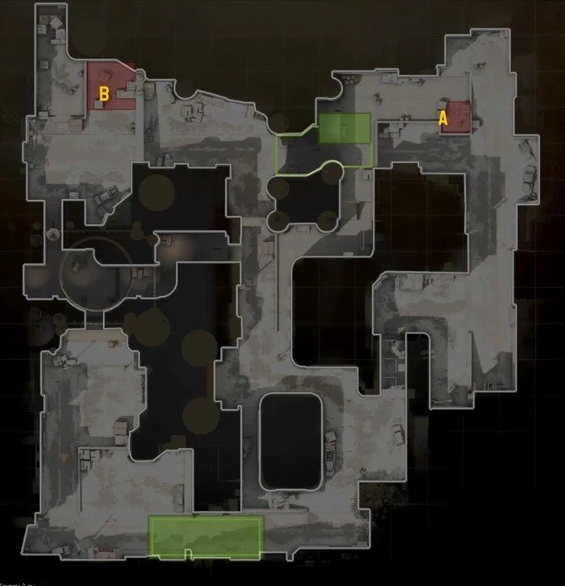
\includegraphics[scale=0.6]{game/map.png}
		\caption{\label{fig:map}Example of Dust2, a CS:GO map}
	\end{figure}
	
	Both these modes need two opposed teams: terrorists and counter-terrorists (shown in Figure \ref{fig:teams}). 
	These teams have some objectives to achieve. 
	During every round, every player earns in-game currency based on single actions (such as kills) or team actions (for example clearing objectives). 
	At the same time, negative actions (such as killing a teammate) leads to losing the in-game money. 
	Every player can use the currency earned in the previous round to buy weapons or other utilities for the current round. 
	
	\begin{figure}[!h] 
		\centering 
		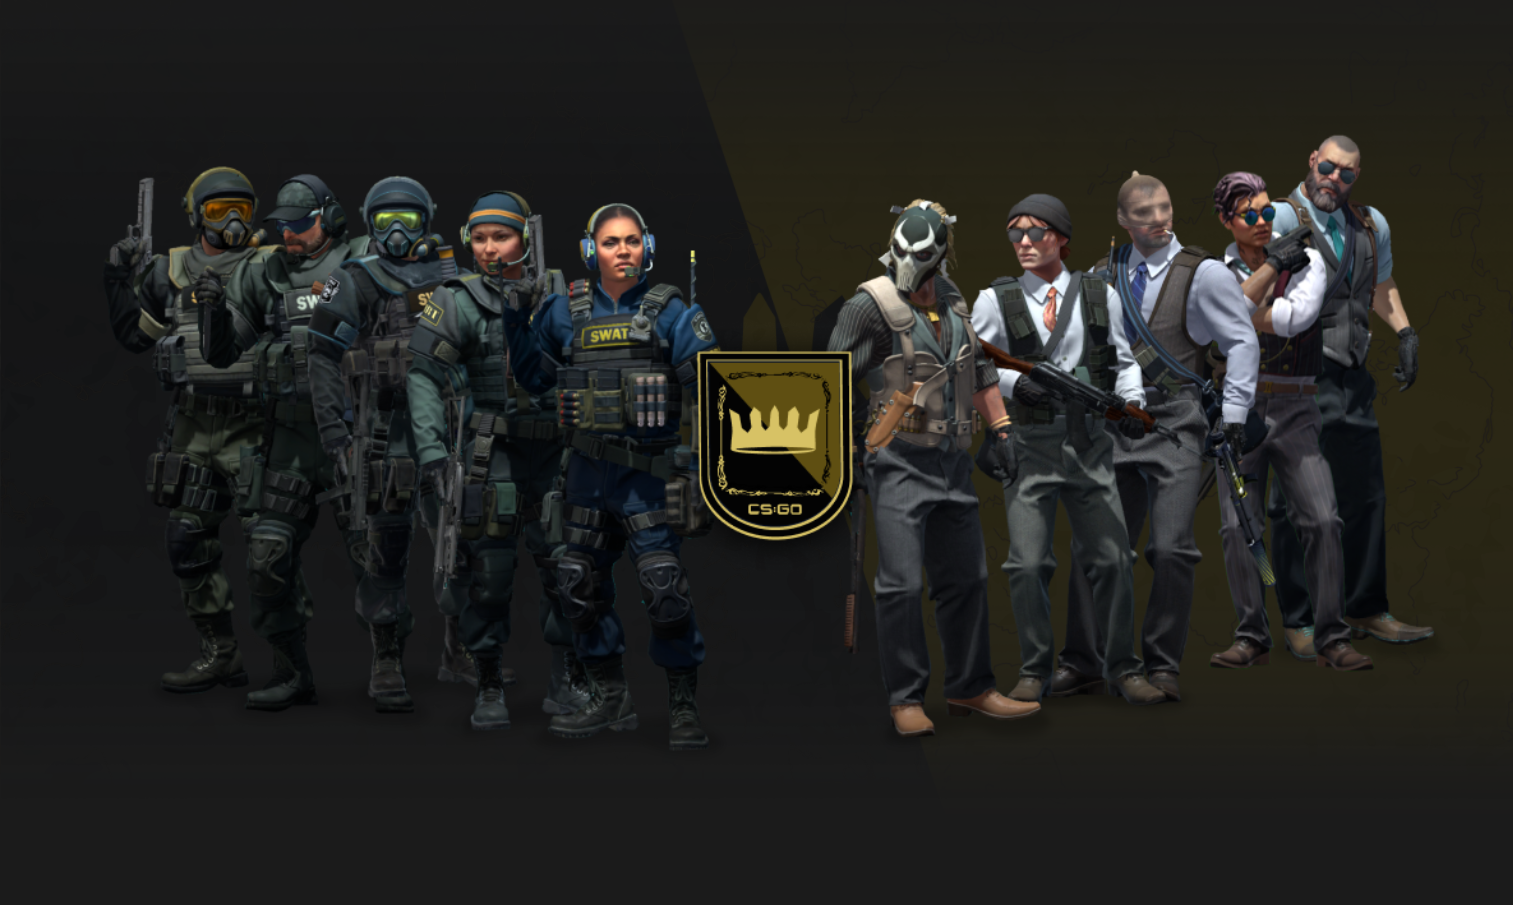
\includegraphics[width=0.9\columnwidth]{game/csgo_teams.png}
		\caption{\label{fig:teams}CS:GO teams: counter-terrorists and terrorists}
	\end{figure}

	In CS:GO, there are nine different maps for competitive play, of which Dust2 (in Figure \ref{fig:map}) is an example. 
	Every map has some predefined spawn points for both terrorists and counter-terrorists. 
	There are also two predefined areas to plant the bomb (labeled as A and B, as previously mentioned) and a predefined extraction point for the hostage scenery.

	\paragraph{\textsc{The match}}\\

		A competitive match is composed of 30 rounds. Every round is divided into two parts:
		
		\begin{itemize}
		
			\item \textbf{The item purchase}:\\
				At the beginning of the match, there is some time dedicated to purchasing, from the in-game store (Figure \ref{fig:store}) the equipment necessary for the round. 
				The purchasing can include better or different weapons or other utilities to win.
			
			\item \textbf{The match}:\\
				The match itself is, of course,  the core part of the game. In this phase, the players try to achieve their objectives. 
				For the terrorists' team, the goal is to plant the bomb and make it explode or prevent the hostages from escaping. 
				On the other side, the counter-terrorists must prevent the bomb from exploding or make the hostages escape. 
				This phase is usually very different in every round and on every map.
			
		\end{itemize}
	
	\begin{figure}[!h] 
		\centering 
		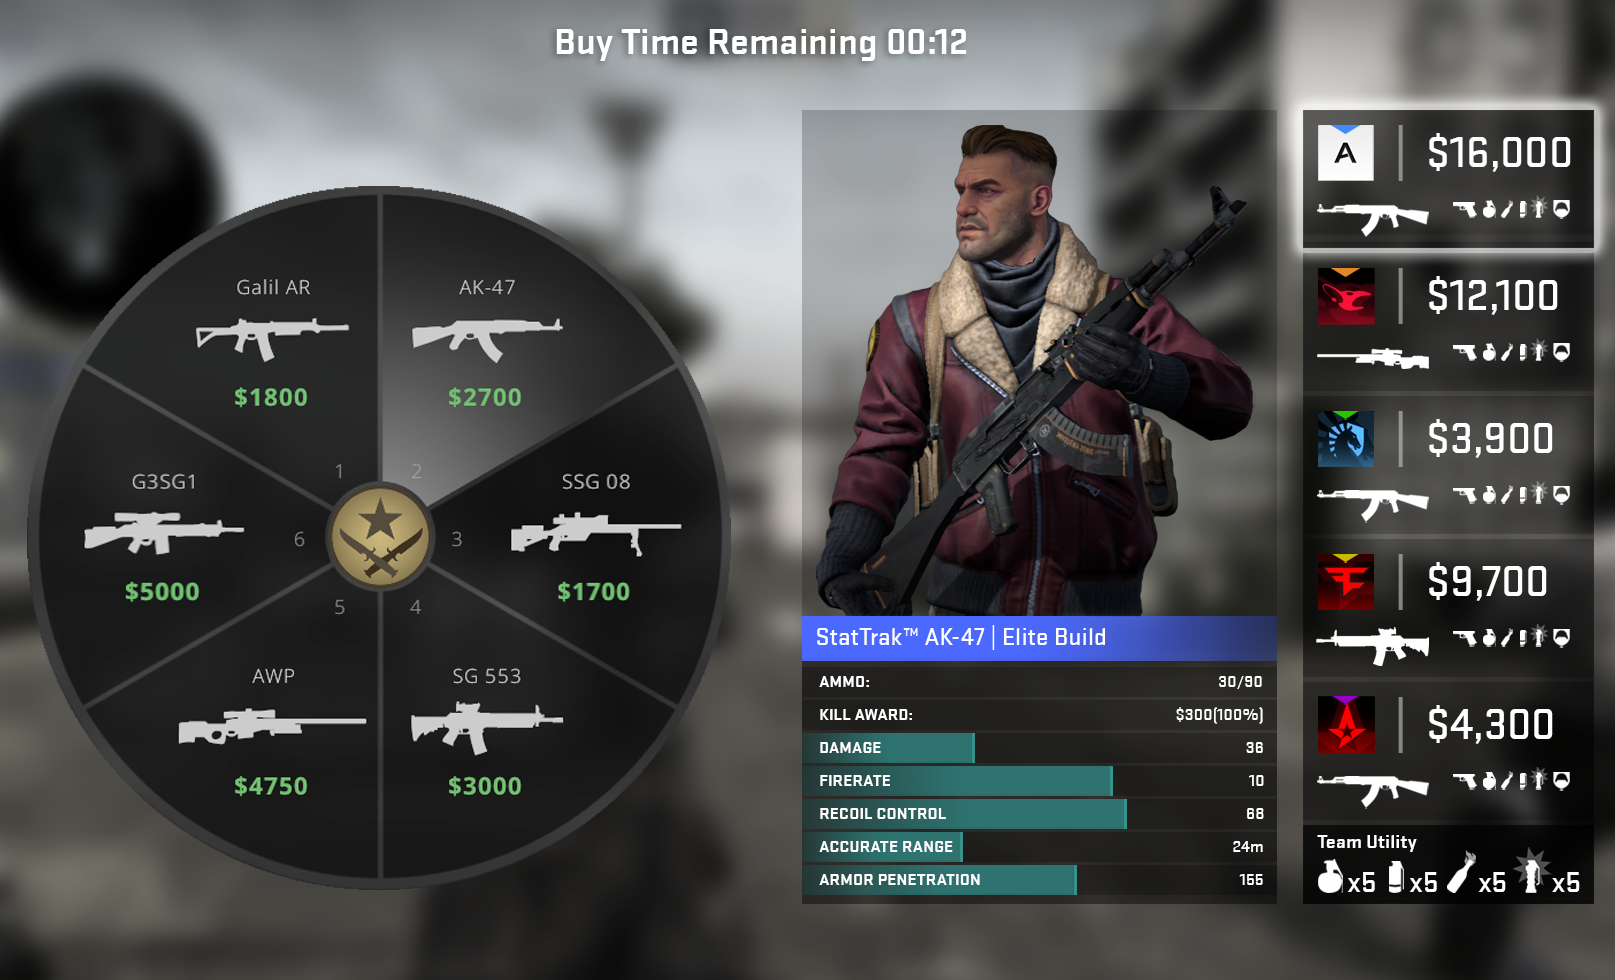
\includegraphics[width=0.9\columnwidth]{game/store.png}
		\caption{\label{fig:store}In-game store example}
	\end{figure}
	
	%\newpage
	
	\subsection{Considerations about the game}
		
		Seeing the gameplay, we thought that this video game was a good candidate for player recognition. 
		Some things that helped us in the educated guess are:
		
		\begin{itemize}
		
			\item The presence of many weapons, divided into six different categories. 
			The personal preference varies for each player and could help in the recognition. 
			\item There are also many possible actions. The number of occurs of every action can help in our task. 
			\item Being an FPS, how each player moves the mouse can be a crucial factor in player recognition.
			\item Most likely also the way one moves can be a major factor in achieving our objective.
		
		\end{itemize} 

%**************************************************************

\section{\label{sec:ml}Machine learning techniques}

	The problem faced is a classification problem. 
	In artificial intelligence, a classification problem is when a machine tries to identify the category of an observation based on previous training. 
	Usually, to achieve this goal, machine learning is a key factor.
	
	\subsection{Model used}
	
		In this chapter, the focus is on presenting the main model used for player recognition.\\
		A powerful class of machine learning algorithms is the one represented by Neural Networks (NN). 
		Neural Networks tries to reproduce biological neural networks, thus are composed of neurons. 
		Artificial Neural Networks' goal is to find patterns in input data, learn from them and generate a corresponding output. 
		Usually, the neurons are organized in ``layers'', which are a set of connected neurons. 
		There are typically three types of layers. 
		These are the input layer (receives data), the hidden layer (finds the patterns), and the output layer (produces results). 
		The connections between the neurons are weighted so that the network can learn only the relevant patterns. 
		The weights are tuned using backpropagation during the training phase.\\
		Figure \ref{fig:nn} shows an example of neural network. 
		
		\begin{figure}[!h] 
			\centering 
			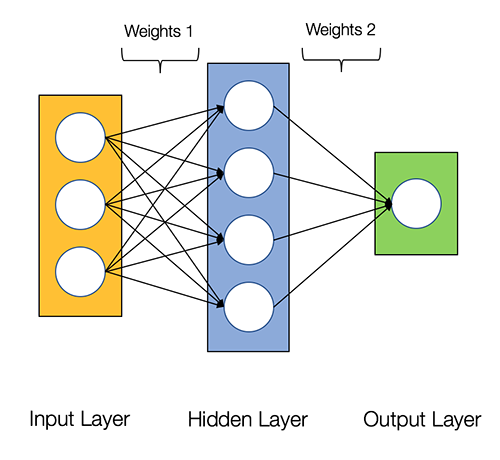
\includegraphics[scale=0.4]{nn/NN.png}
			\caption{\label{fig:nn}Example of neural network}
		\end{figure}
		
		\newpage
		
		A neural network is ``deep'' if there is more than one hidden layer. 
		Deep neural networks are usually used because can understand more complex patterns. 
		A particular deep learning neural network is the Recurrent Neural Network (RNN), which can work with sequences and learn temporal patterns. 
		This peculiarity is achieved with a particular structure of the hidden layer. 
		The information gets stored in the hidden layer and passed to the following one. 
		It can be seen as multiple copies of one neural network, each one passing a message to the following one.\\
		Figure \ref{fig:rnn} shows an RNN, where $A$ is the network, $x_i$ si the input at time $i$ and $h_i$ is the output at time $i$.
		
		\begin{figure}[!h] 
			\centering 
			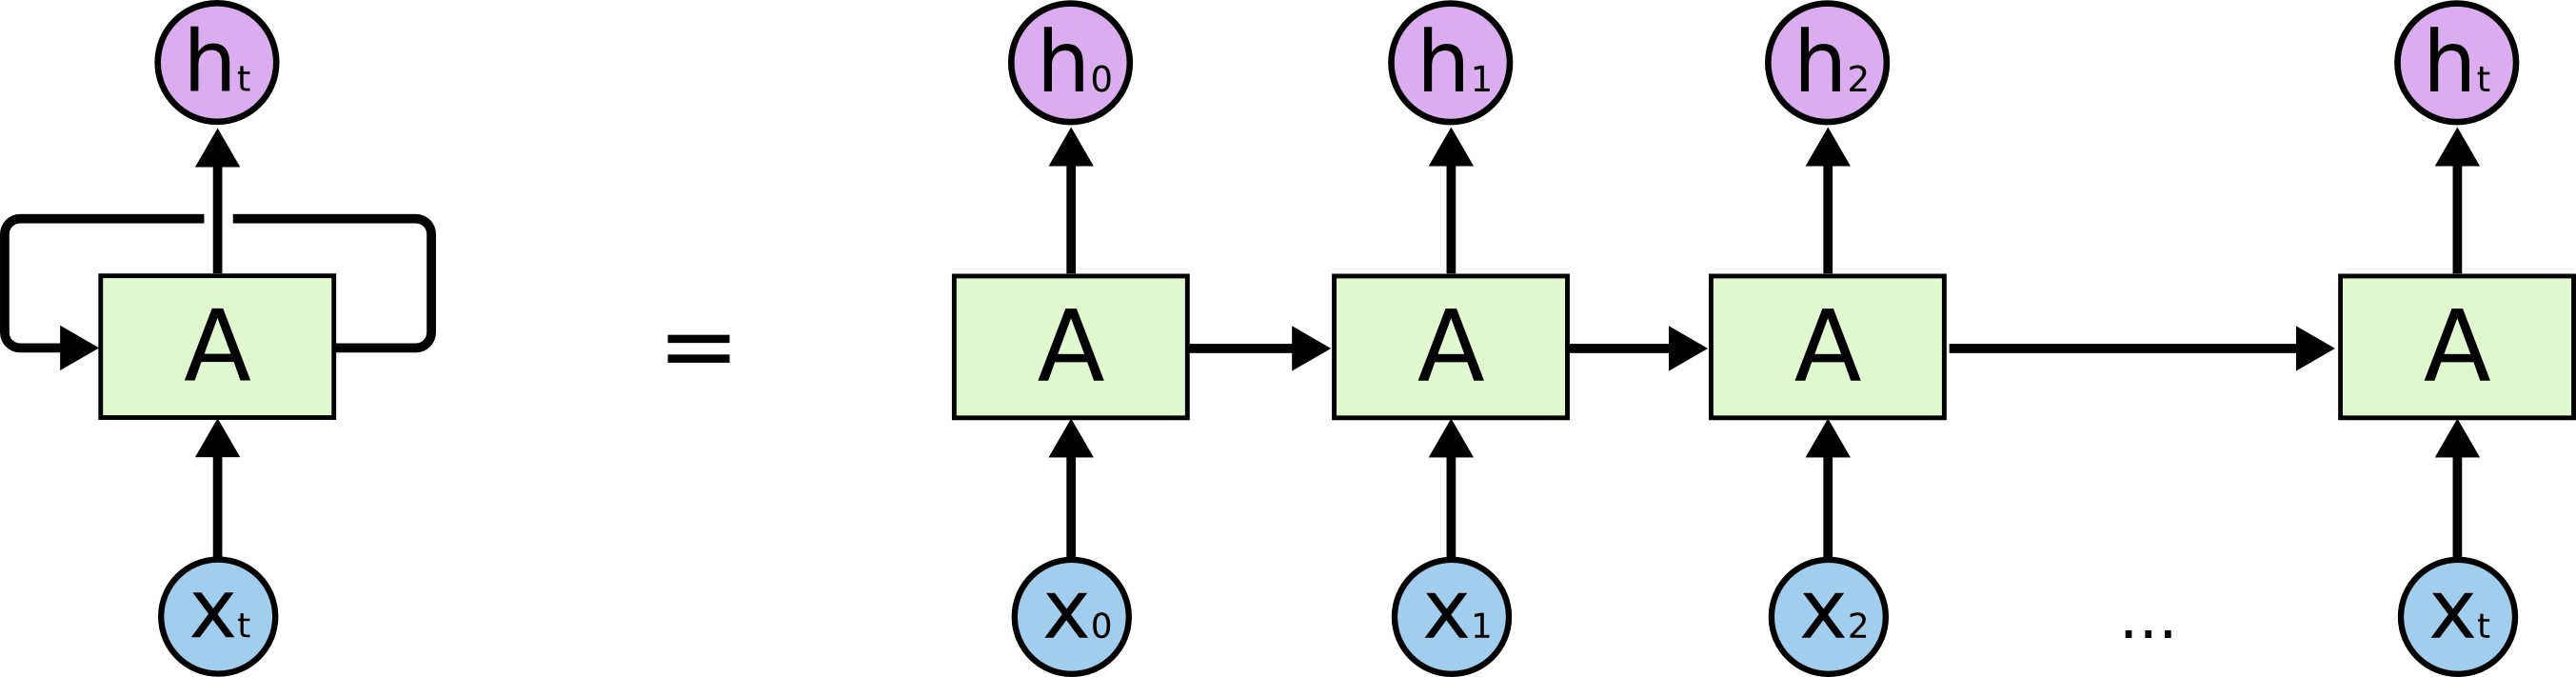
\includegraphics[width=0.9\columnwidth]{nn/RNN.png}
			\caption{\label{fig:rnn}Example of a RNN.}
		\end{figure}
		
		Formally, a Recurrent Neural Network is defined as: \\
		
		\begin{center}
			\begin{equation}
				\begin{aligned}
					$h_t\ =\ \phi (W \ \cdot \ x_t \ + \ U \ \cdot \ h_{t-1})$ \label{for:rnn} \noalign{\vskip1pt}
				\end{aligned}
			\end{equation}
		\end{center}
		
		where W and U are the weight matrix and the transition matrix respectively. 
		$\phi$ is the activation function. 
		The two matrices are used to determine which and how important is the information in the hidden layers. 
		RNN can be very useful, but there are two problems with this kind of neural network. 
		These two problems are known as ``exploding gradient'' and ``vanishing gradients''~\cite{REHMER20201243}. 
		These 2 problems are both resolved using Long Short Term Memory (LSTM)~\cite{10.1162/neco.1997.9.8.1735}.
		This type of neural network is organized in cells (shown in Figure \ref{fig:cell})
		
		\begin{figure}[!h] 
			\centering 
			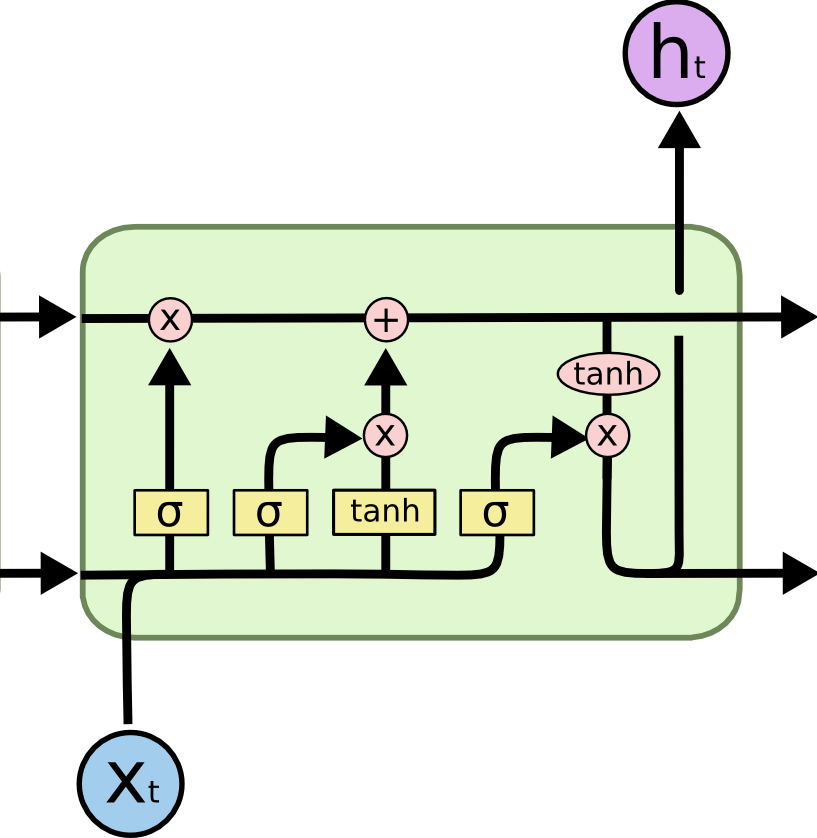
\includegraphics[scale=.35]{nn/LSTM.png}
			\caption{\label{fig:cell}Example of a LSTM cell}
		\end{figure}
		
		The solution to the two mentioned problems is represented by the structure of the cells. 
		There are three structures called gates that control the input and help achieve this goal.
		The gates' name are forget gate, input gate and output gate.
		
		\begin{figure}[!h] 
			\centering 
			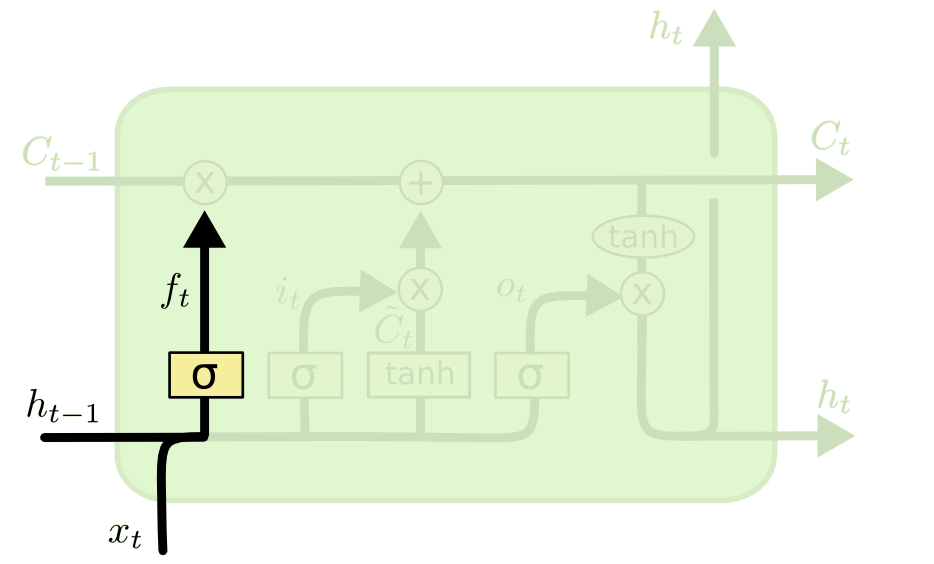
\includegraphics[scale=.7]{nn/LSTM_step1.png}
			\caption{\label{fig:step1}First step of a LSTM neural network}
		\end{figure}
		
		In Figure \ref{fig:step1} is shown how the LSTM uses the forget gate to decide what to forget about the cell state.
		The formula used is:
		\begin{center}
			\begin{equation}
				\begin{aligned}
					$f_t\ =\ \sigma (W_f\ \cdot \ [h_{t-1}, x_t] + b_f)$, \label{for:fg}\noalign{\vskip1pt}
				\end{aligned}
			\end{equation}
		\end{center}
		
		where $h_{t-1}$ is the output of the previous cell, $x_t$ is the input at time $t$, $W$ is the weight matrix, and $b_f$ is the bias vector.
		The output value, scaled between 0 and 1 with a sigmoid function, helps to understand how much to consider from the previous state. 
		
		\begin{figure}[!h] 
			\centering 
			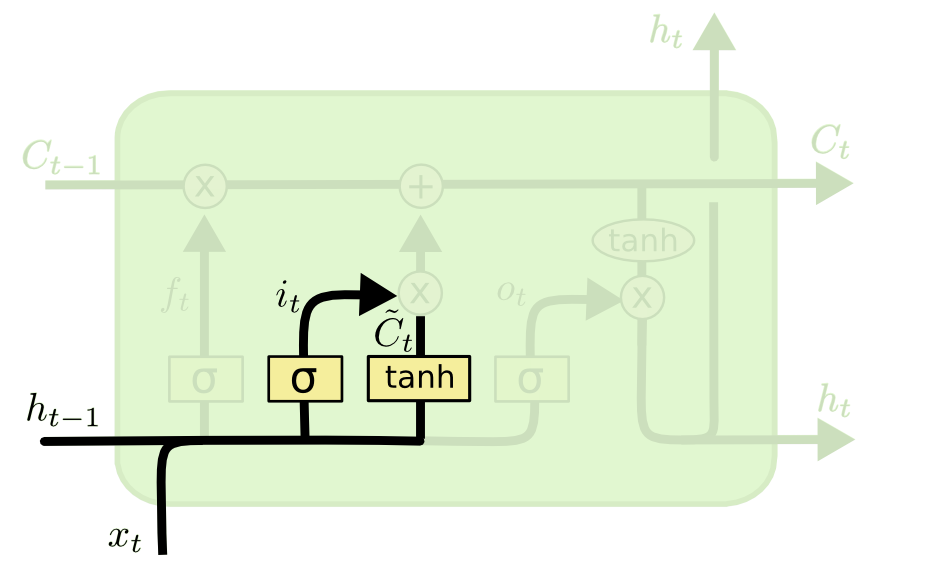
\includegraphics[scale=.7]{nn/LSTM_step2.png}
			\caption{\label{fig:step2}Second step of a LSTM neural network}
		\end{figure}
		
		Figure \ref{fig:step2} shows the second step of the forward propagation of a LSTM cell.
		First, a sigmoid layer (the input gate) decides what to update using the following formula:
		
		\begin{center}
			\begin{equation}
				\begin{aligned}
					$i_t\ =\ \sigma (W_i\ \cdot \ [h_{t-1}, x_t] + b_i)$ \label{for:ig}\noalign{\vskip1pt}
				\end{aligned}
			\end{equation}
		\end{center}
		
		Next, a $\tanh$ layer creates a new vector of candidate values. 
		The candidates values, identified with $\tilde{C_t}$, are computed as:
		
		\begin{center}
			\begin{equation}
				\begin{aligned}
					$\tilde{C_t}\ =\ \tanh (W_C\ \cdot \ [h_{t-1}, x_t] + b_C)$ \label{for:ig2}\noalign{\vskip1pt}
				\end{aligned}
			\end{equation}
		\end{center}
		
		\begin{figure}[!h] 
			\centering
			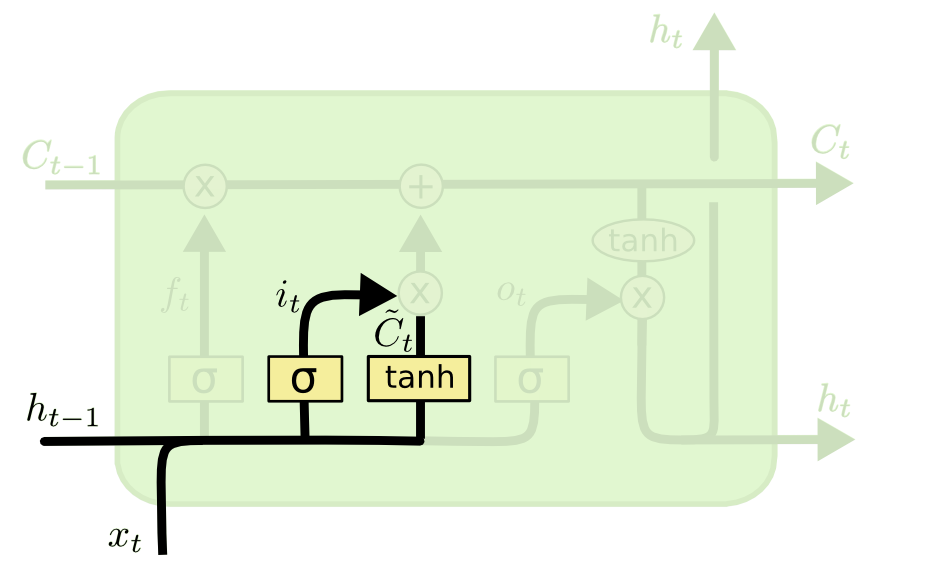
\includegraphics[scale=.7]{nn/LSTM_step2.png}
			\caption{\label{fig:step3}Third step of a LSTM neural network}
		\end{figure}
		
		Figure \ref{fig:step3} shows how the state of the cell changes. 
		First the previous cell state gets multiplied by the output of the forget gate with an element-wise operation.
		Second the values calculated in \ref{for:ig} and \ref{for:ig2} gets multiplied with another element-wise operation and then added to the state cell.
		The formula that can summarize this operation is:
		
		\begin{center}
			\begin{equation}
				\begin{aligned}
					$C_t\ =\ \tanh (f_t\ \cdot \ C_{t-1} + i_t\ \cdot \ \tilde{C_t})$ \label{for:add}\noalign{\vskip1pt}
				\end{aligned}
			\end{equation}
		\end{center}
		
		\begin{figure}[!h] 
			\centering 
			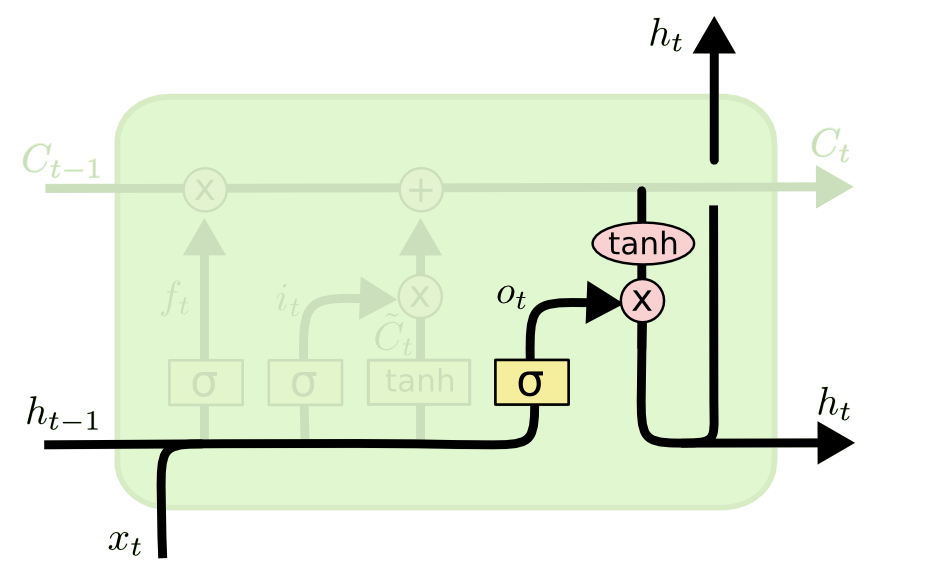
\includegraphics[scale=.7]{nn/LSTM_step4.png}
			\caption{\label{fig:step4}Fourth step of a LSTM neural network}
		\end{figure}
		
		Lastly, figure \ref{fig:step4} shows how the cell decide what to output.
		First, a sigmoid layer decides what to output.
		Then a $\tanh$ layer scales all the values of the cell state between $-1$ and $1$.
		Finally the network performs an element-wise multiplication of the cell state and the output of the sigmoid layer. 
		This process can be summarized with the following formulas:\noalign{\vskip1pt}
		\begin{center}
			\begin{equation}
				\begin{aligned}
					$o_t\ = \ \sigma(W_0 [h_{t-1}, x_t] + b_o)$\\ \noalign{\vskip1pt}
				\end{aligned}
			\end{equation}
		\end{center}
		\begin{center}
			\begin{equation}
				\begin{aligned}
					$h_t\ = \ o_t \ \cdot \ \tanh(C_t)$\noalign{\vskip1pt}
				\end{aligned}
			\end{equation}
		\end{center}
		
	\subsection{Loss function}
	
		During the learning process it is the goal of the model to find the best solution. 
		To find the best solution the model evaluates an ``objective function'' and in this particular task we want to minimize the error of the predictions. 
		In order to achieve this goal the objective function, called ``loss'' function, is directly proportional to how much the predicted results differs from the actual result.\\
		In this classification task, given that every sample can be part of only one class, we chose to use a loss function known as Categorical Crossentropy Loss Function.
		Formally this function is defined as:
		
		\begin{center}
			\begin{equation}
				\begin{aligned}
					$L(y, \hat{y})\ = \ -\displaystyle\sum_{j=0}^M \displaystyle\sum_{i=0}^N (y_{ij} * \log (\hat{y_{ij}})) $\noalign{\vskip1pt}
				\end{aligned}
			\end{equation}
		\end{center}
		
		In this formula, $\hat{y}$ is the predicted value, $i$ is the training sample, $j$ is the output node. $\hat{y_{ij}}$ is the prediction of the sample $i$ belonging to the class $j$ and 
		$y_{ij}$ is the actual value. \\

		The categorical crossentropy loss function compares the distributions of the predictions (the predictions of the output layer, one for each class) with the true distribution, where the 
		probability of the true class is 1 and 0 for every other class. 
		The true classes are simply represented as a one-hot encoded vectors, with only one 1 in the true class and 0 elsewhere, and the closer the model’s outputs are to those vectors, the lower the loss is.
	
	\subsection{Metrics adopted}
	
		In this elaborate, we will use some of the most common metrics to evaluate our models: accuracy and precision.
		In Table \ref{tab:cm} is presented a confusion matrix that will help us to describe the mentioned metrics.
	
		\begin{table}[!h]
			\caption{\label{tab:cm}Confusion matrix}
			\centering
			\begin{tabular}{l|l|c|c|}
				\multicolumn{2}{c}{}&\multicolumn{2}{c}{\textbf{Predicted}}\\
				\cline{3-4}
				\multicolumn{2}{c|}{}&\textbf{Positive}&\textbf{Negative}\\
				\cline{2-4}
				\multirow{\textbf{Actual}}& \textbf{Positive} & True positive & False negative \\
				\cline{2-4}
				& \textbf{Negative} & False positive & True negative\\
				\cline{2-4}
			\end{tabular}
		\end{table}
		
		\paragraph{Accuracy}: Accuracy is defined as:
		
			\begin{center}
				\begin{equation}
					\begin{aligned}
						$Accuracy = \dfrac{TP + TN}{FP + TP + TN + FN}$ \noalign{\vskip1pt}
					\end{aligned}
				\end{equation}
			\end{center}
		
			This metric measures the model's performance considering true positives and true negatives against all the dataset's examples.
			A low value indicates a significant difference between predictions and target values. 
		
		\paragraph{Precision}: Precision is defined as:
		
			\begin{center}
				\begin{equation}
					\begin{aligned}
						$Accuracy = \dfrac{TP}{FP + TP}$ \noalign{\vskip1pt}
					\end{aligned}
				\end{equation}
			\end{center}
		
			This metric measures how many of the predicted true values are truly positive. 
			It helps to determine if the classification error with respect to the true positive is high.             % Kick-Off
% !TEX encoding = UTF-8
% !TEX TS-program = pdflatex
% !TEX root = ../tesi.tex

%**************************************************************
\chapter{Data collection}
\label{cap:analisi-requisiti}
%**************************************************************

\intro{This chapter gives an overview of the data collection process, which finished with the creation of the logs that we used as base for our work.\\ 
In section \ref{sec:fi} we present the process of finding the data, in section \ref{sec:do} we look at the way the matches were downloaded, and in section \ref{sec:pa} we explore the parsing.}

%***************************************************************

\section{\label{sec:fi}Finding the data}

	The first step of the data collection was to find a tracking website that could provide the replays of the matches. 
	For this purpose, the two websites considered are csgostats\footnote{\href{https://csgostats.gg/}{https://csgostats.gg/}} and hltv\footnote{\href{https://www.hltv.org/}{https://www.hltv.org/}}.
	In the beginning, csgostats seemed a better choice, so, looking through the players, 50 of them were selected. 
	Every selected player must have played at least 100 matches as the minimum requirement. 
	After we found the profiles, we tried to create a script to download the matches automatically. 
	The problem was that there is the invisible reCAPTCHA, so we decided to use hltv, which does not use these codes. 
	After that, we checked if the players selected were present in hltv. 
	We then replaced the players that were not present on this website with other players that we found. 
	As the final step, we wrote all the links to the profiles of the players on hltv on a \emph{txt} file.

\section{\label{sec:do}Getting the data}

	For every player we found, we had to download 100 matches. 
	We found a way to automate the download process with a python script and the framework Selenium\footnote{\href{https://www.selenium.dev/}{https://www.selenium.dev/}}. 
	Using Selenium's Chrome web driver, we downloaded all the matches starting from the profile page of one player at a time. 
	The download starts when the web driver performs a request, via Selenium's get method, to a link for the direct download of the replay. 
	The download result is a compressed file that gets unpacked using the pyunpack module\footnote{\href{https://github.com/ponty/pyunpack/tree/0.2.2}{https://github.com/ponty/pyunpack/tree/0.2.2}}. 
	The extracted files get counted and renamed to keep track of how many matches remain to reach 100. 
	Finally, the compressed archives get deleted from the pc.

\section{\label{sec:pa}Parsing the matches}

	The parsing process is divided into two parts: the modification of the parser itself to parse what we needed and the automation of the parsing process.
	To parse the data we needed, we first found an already existing parser. 
	The mentioned parser is called demoinfogo and is an open-source software developed by Valve. 
	In the beginning, we parsed a match with the original parser to see the result. 
	Then we modified the outputs to trace the origin of every line in the output file. 
	After that, we changed the parser, silencing what we did not need and writing in a file everything relevant for our task. 
	Lastly, we wrote a python script that helped us automatically parse all the matches and rename all the files with the corresponding player's name. 
	These files created by the parser are the logs we used as starting point in this work.

	In more detail, the fundamental unit of the replay is the \gls{tick}, and the parser dumps the state of every player and every action occurred during the tick with the related informations. 
	So, the parsed replay can be seen as a sequence of states dumped by the parser. 
	The states can include both player information and actions informations.
	Figure \ref{fig:act} presents an example of parsed action.
	
	\begin{figure}[!h] 
		\centering 
		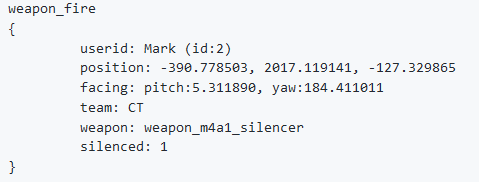
\includegraphics[width=.9\columnwidth]{parser/original_action.png}
		\caption{\label{fig:act}Example of parsed action.}
	\end{figure}
	
	Given this, we used the parser to dump only a set of features (shown in Table \ref{tab:fea}) of the player we were interested in.
	
	\begin{table}
	
		\caption{\label{tab:fea}List of parsed features}
		\centering
		\begin{tabular}{|c|c|}
		
			\hline
			\textbf{Type} & \textbf{Features}\\
			\hline
			Camera & X, Y \\
			\hline
			Player position & X, Y, Z \\
			\hline
			door\_moving & occurred \\
			\hline
			player\_blind & occurred, blind\_duration \\
			\hline
			round\_mvp & occurred \\
			\hline
			defuser\_pickup & occurred \\
			\hline
			bomb\_pickup & occurred \\
			\hline
			defuser\_dropped & occurred \\
			\hline
			bomb\_dropped & occurred \\
			\hline
			bomb\_abortdefuse & occurred \\
			\hline
			bomb\_begindefuse & occurred \\
			\hline
			bomb\_abortplant & occurred \\
			\hline
			bomb\_beginplant & occurred \\
			\hline
			bomb\_defused & occurred \\
			\hline
			bomb\_planted & occurred \\
			\hline
			bullet\_impact & occurred \\
			\hline
			weapon\_zoom & occurred \\
			\hline
			weapon\_zoom\_rifle & occurred \\
			\hline
			player\_falldamage & occurred, damage\\
			\hline
			molotov\_detonate & occurred \\
			\hline
			tagrenade\_detonate & occurred \\
			\hline
			hegrenade\_detonate & occurred \\
			\hline
			flashbang\_detonate & occurred \\
			\hline
			item\_purchase & occurred, item\_purchased \\
			\hline
			ammo\_pickup & occurred \\
			\hline
			silencer\_detach & occurred \\
			\hline
			decoy\_detonate & occurred \\
			\hline
			smokegrenade\_detonate & occurred \\
			\hline
			weapon\_fire & occurred, weapon \\
			\hline
			weapon\_reload & occurred \\
			\hline
			player\_jump & occurred \\
			\hline
			player\_death & occurred, type (kill, death, or assist)\\
			\hline
			item\_pickup & occurred, item\_picked \\
			\hline
			item\_equip & occurred, item\_equipped\\
			\hline
	
		\end{tabular}
	
	\end{table}

	In this way, viewing the replay as a sequence of states and the parser as a program used to dump those states, we could parse the replays.
	So, the parser dumps the replays in a predefined way, following this structure:
	
	\begin{itemize}
	
		\item If the parser has to dump an action, it writes the word Action, the tick when the action occurred, the action name, and then the additional informations (if present)
		\item If the parser has to dump the player's state, it writes the word Entity, the current tick, the mouse position ($X$ and $Y$), the player's position in the map ($X$, $Y$, and $Z$), 
		the player's velocity ($X$, $Y$, and $Z$), and the Y offset (used to determine the crouch state).
	
	\end{itemize}
	
	In Figure \ref{fig:parsed} there is an example of a parsed match.
	
	\begin{figure}[!h] 
		\centering 
		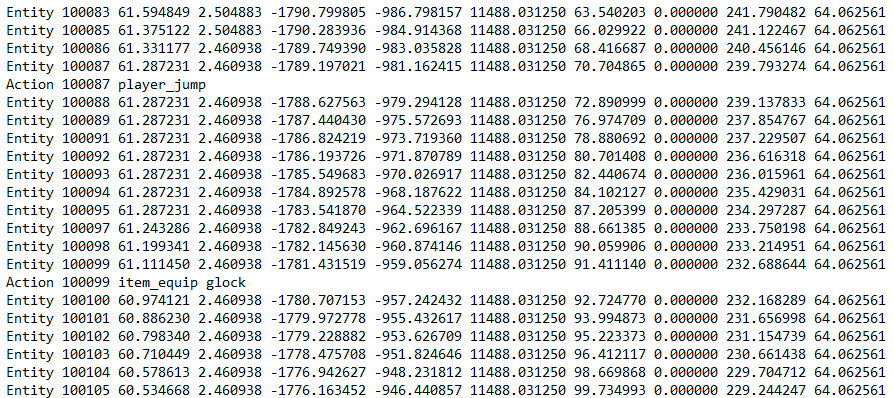
\includegraphics[width=0.9\columnwidth]{parser/log.png}
		\caption{\label{fig:parsed}Parsed replay fragment.}
	\end{figure}

	For more details on the parser see appendix \ref{app:par}
             % Concept Preview
% !TEX encoding = UTF-8
% !TEX TS-program = pdflatex
% !TEX root = ../tesi.tex

%**************************************************************
\chapter{Our work}
\label{cap:progettazione-codifica}
%**************************************************************

\intro{In this chapter we present what we did. In section \ref{sec:pre} we present the preprocessing of the logs and in section \ref{sec:exp} we cover the experiments we performed.}

%**************************************************************

\section{\label{sec:pre}Preprocessing}

	\subsection{Data cleaning}
		The first thing we did was cleaning the data. 
		This operation was necessary because the parser parsed also the prematch. 
		This part of the game would have been a problem because the players usually do not move and the vision does not move even if the player moves the mouse. 
		Moreover, there is some time, during which the players cannot move.
		That would result in any player stopping for the prematch's amount of time.
		This caused the necessity to clean the data to remove the prematch from the parsed log.
	
	\subsection{\label{sec:cut}Match cutting}
		Given that the matches can be very long and that can have different durations, we decided to cut them and keep only the first ten minutes of every game. 
		It was easy to understand where to cut the file because the parser we used wrote, in every line, the corresponding \gls{tick}. 
		Knowing how many ticks per second there are in the game, we were able to calculate how many ticks we had to keep in the log and cut the file accordingly.
		
	\subsection{Sequence creation}
		We had 100 matches for each player, and after cutting them, we had only the first ten minutes of every game. 
		In our task, the less time we need for reliable identification, the better. 
		So we decided to divide each log into 5 parts, each one corresponding to a sequence of two minutes of gameplay. 
		To achieve this, we used the same method described in \ref{sec:cut}, using the ticks as guidelines. 
		
	\subsection{Interpolation}
		
		We noticed that the parser had a problem concerning the creation of the logs. 
		The logs are made of dumps that occur every two ticks. 
		Sometimes, though, there were some missing ticks.
		We had to find a way to deal with the missing data. 
		Given that the missing data were not many, we decided to interpolate them.
		This solution is widely used to deal with missing data in sequences and allows to keep the behaviours if the missing data are a few compared to the entire sequence, and that happened to be our case. 
		If there was only one tick to be interpolated, so there was a four ticks difference between two lines, the interpolation was done computing the mean of the previous and the successive tick. 
		In case there were multiple missing ticks, we chose to interpolate in the same way. 
		That has the effect of making it look like the player exponentially slows down the movement. 
		We thought this could be a plausible behaviour, mainly because the player's motions try to be as precise as possible, so the players may slow down the movement when they comes close to their objective.
	
	\subsection{Data aggregation}
		
		The following step is data aggregation. 
		A crucial decision is how many ticks to aggregate. 
		With DOTA 2, the decision was to aggregate 15 ticks. 
		This decision resulted in aggregating portions of gameplay with a duration of half a second. In our work, we did some experiments to understand which one was the best option. 
		In CS:GO, there are 64 ticks in a second, so we tried to aggregate 16 and 32 ticks, corresponding respectively to a quarter and half a second. 
		In the following images, some graphs can help to understand the difference between the two options. 
		The first graph, in Figure \ref{fig:gr0}, shows the trend of the player's speed along the z-axis, of one of the matches.
		
		\begin{figure}[!h] 
			\centering 
			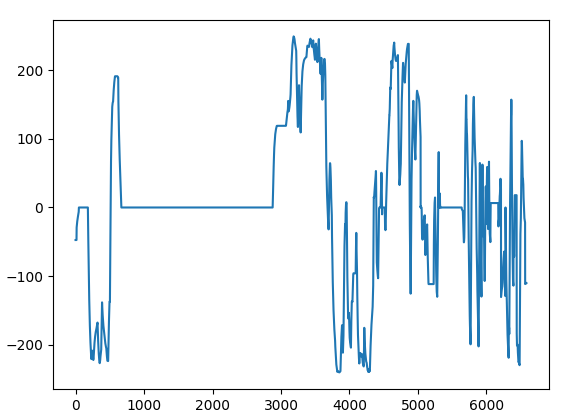
\includegraphics[scale=.7]{grafici/Grafico 2.png}
			\caption{\label{fig:gr0}Graph of the player's speed along the z axis.}
		\end{figure}
		
		In figure \ref{fig:gr1}, we can see the same data. 
		The only difference is that the second image presents the log after the aggregation process occurred.
		This graph shows the result of the trend after a 16-ticks-aggregation. 
		In figure \ref{fig:gr2}, we can see the same chart after a 32-ticks-aggregation. 
		
		\begin{figure}[!h] 
			\centering 
			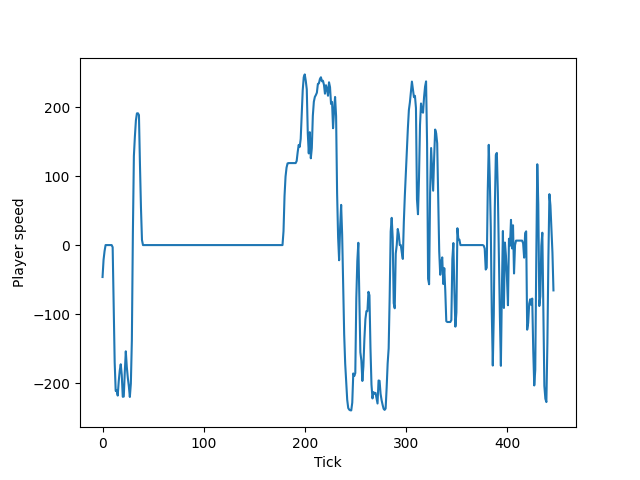
\includegraphics[scale=.7]{grafici/Grafico 3.png}
			\caption{\label{fig:gr1}Graph of the player's speed along the z axis after a 16-ticks aggregation.}
		\end{figure}
		
		\begin{figure}[!h] 
			\centering 
			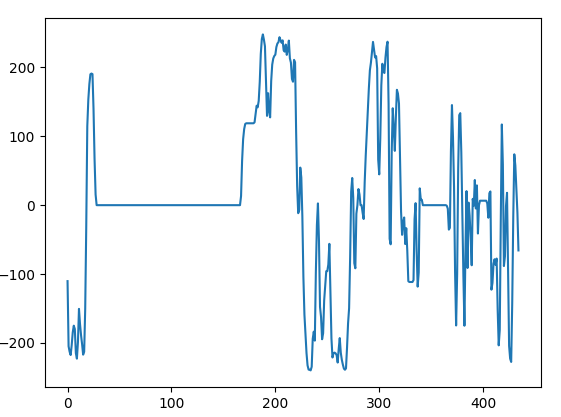
\includegraphics[scale=.7]{grafici/Grafico 4.png}
			\caption{\label{fig:gr2}Graph of the player's speed along the z axis after 32-ticks aggregation.}
		\end{figure}
		
		As shown in the previous images, there is a difference in aggregating with 16 or 32 ticks. 
		Of course, the graph shows only one data sequence, but we did not base our decision only on the information we could retrieve from this single graph. 
		The decision was taken after studying the differences in distributions of the values to identify the best number of ticks to aggregate, 
		using the Kolmagorov-Smirnov statistics to quantify the distance between the raw data and the aggregated data, as shown in Quantifying Information Loss Through Data Aggregation~\cite{womak:info_loss}.
		The candidate values were $16$ and $32$, because any number lower than $16$ would have been not enough to reduce memory usage and any number higher than $32$ would result in losing too much information. 
		After evaluating both the candidate values, although the difference is not very big, we decided it would have been better to use the 16-ticks-aggregation because it results in a lower information loss. 
		
		
	\subsection{Split creation}
	
		The following step was to split the dataset into three sets: the training set, the validation set, and the test set. 
		We decided to use an 80\%-10\%-10\% split. 
		The dataset was split as part of the preprocessing to avoid the model using the test set in some of the epochs as part of the training and to avoid computing a split every time we ran the neural network training script.
		
	\subsection{Standardization}

		To save time in the training process, we decided to standardize all the logs as part of the preprocessing phase. We decided to use the standard scaler provided by sklearn\footnote{\href{https://scikit-learn.org/stable/modules/generated/sklearn.preprocessing.StandardScaler.html}{https://scikit-learn.org/stable/modules/generated/sklearn.preprocessing.StandardScaler.html}}. 
		This scaler needs to be fit on the data, and we decided to do so using the training split. 
		The result is that the training split was scaled in the range $[-1, 1]$, while the validation and test split were scaled but not necessarily in the $[-1, 1]$ range. 
		This decision was taken to avoid overfitting problems, due to the fact that we do not know what data we can find in the validation or test set.

%**************************************************************

\section{\label{sec:exp}Experiments}

	\subsection{First model}
			
		In our work, just as DOTA 2, we decided to use a Recurrent Neural Network, specifically a Long Short Term Memory (LSTM). 
		This decision was almost mandatory because we worked with sequences and because the time information is relevant. 
		LSTM is, in fact, a type of neural network in which information persists in time. 
		For instance, an LSTM neural network can learn the pattern followed by a specific player in the movements on the map, while a simple neural network cannot.
		Following the same intuition behind the DOTA 2 work, we thought that some actions, such as the camera movements, can be biometric, meaning that everyone has a different way to do it.\\
		
		
		In our model, there are two LSTM layers with $\tanh$ activation function, a fully connected layer with $RELU$ activation  function, and a $softmax$ output layer.
		%In the final model there are also two Dropouts layer, with a $0.2$ rate, one after each LSTM layer, even though they were not present in the first model we used.
		The LSTM layers have 256 units each, while the first fully connected layer has 128 units. 
		The output layer has 50 units, due to the number of classes we had. 
		We used a batch size of 128, 100 epochs of training, and the categorical crossentropy loss function. 
		The optimizer we chose is Adam, with a learning rate of $0.01$. 
		Figure \ref{fig:mod1} shows a summary of our model. 
		For the implementation, we used the Keras\footnote{\href{https://keras.io/}{https://keras.io/}} library with a Tensorflow\footnote{\href{https://www.tensorflow.org/}{https://www.tensorflow.org/}} backend. 
		The GPU we used is an Nvidia GeForce GTX 1050 2Gb.
		
		\begin{figure}[!h] 
			\centering 
			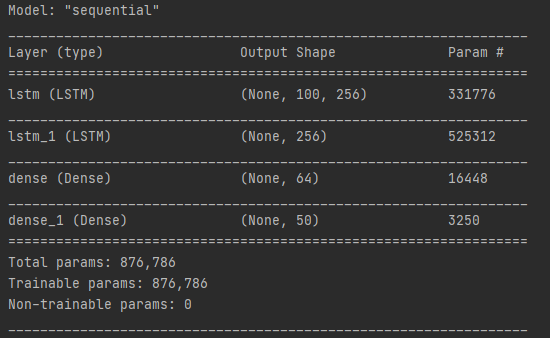
\includegraphics[scale=.6]{modelli/primo_modello.png}
			\caption{\label{fig:mod1}Summary of the first model used.}
		\end{figure}
		
		This first model reached $\sim 0.8$ accuracy and $\sim 0.75$ precision on the validation set. 
		
	\subsection{Feature selection}
	
		The first model we coded had surprisingly high accuracy and precision. 
		Then we tried to eliminate a set of features so that the model could learn better. 
		We used our intuition to identify some features that could introduce noise in the predictions. 
		We thought that the mean of the position on the map could introduce some noise since it depends on the map chosen for the match. 
		Speaking of actions, we noticed that some of the parsed actions were never triggered and, after some researches, we found that the game itself never triggered such events. 
		Given the situation, we decided to ignore these actions, such as the action $door\_moving$. 
		In Table \ref{tab:features} there is a list of the features we kept. 
		
		\begin{longtable}{|c|c|}

			\caption{\label{tab:features}Features we kept after the feature selection process}

			\hline
			\textbf{Type} & \textbf{Features} \\
			\hline
			Mouse position (x axis) & Mean, standard deviation, changes in positive, changes in negative\\
			\hline
			Mouse position (y axis) & Mean, standard deviation, changes in positive, changes in negative\\
			\hline
			Player position (x axis) & Standard deviation, changes in positive, changes in negative\\
			\hline
			Player position (y axis) & Standard deviation, changes in positive, changes in negative\\
			\hline
			Player position (z axis) & Standard deviation, changes in positive, changes in negative\\
			\hline
			Player velocity (x axis) & Mean, standard deviation, changes in positive, changes in negative\\
			\hline
			Player velocity (y axis) & Mean, standard deviation, changes in positive, changes in negative\\
			\hline
			Player velocity (z axis) & Mean, standard deviation, changes in positive, changes in negative\\
			\hline
			Crouch changes & n\_occurs\\
			\hline
			Weapon fire & n\_occurs \\
			\hline
			Weapon reload & n\_occurs \\
			\hline
			Player jump & n\_occurs \\
			\hline
			Kills & n\_occurs \\
			\hline
			Assists & n\_occurs \\
			\hline
			Item pickup & n\_occurs \\
			\hline
			Item equip & n\_occurs \\
			\hline
			Grenade detonate  & n\_occurs \\
			\hline
			Smokegrenade detonate & n\_occurs \\
			\hline
			Molotov detonate & n\_occurs \\
			\hline
			Flashbang detonate & n\_occurs \\
			\hline
			Tagranade detonatoe & n\_occurs \\
			\hline
			Hegranade detonate & n\_occurs \\
			\hline
			Decoy detonate & n\_occurs \\
			\hline
			Player falldamage & n\_occurs \\
			\hline
			Ammo pickup & n\_occurs \\
			\hline
			Silencer detach & n\_occurs \\
			\hline
		\end{longtable}
	
	\subsection{Model selection}
	
		The following runs of the training script resulted in a better-performing neural network. 
		We could easily reach 90\% accuracy and precision in both the validation and test set, as shown in figures \ref{fig:acc1} and \ref{fig:acc2}.
		We were also able to stabilize the loss as shown in Figure \ref{fig:loss1} and \ref{fig:loss2}.
		
		\begin{figure}[!h]
			\centering
			\begin{minipage}{.5\textwidth}
				\centering
				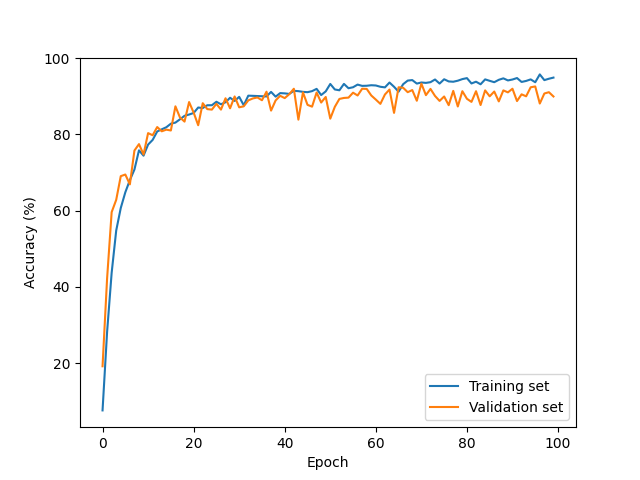
\includegraphics[width=.8\linewidth]{risultati/accuracy.png}
				\caption{\label{fig:acc1}Training and \\ validation accuracy}
			\end{minipage}%
			\begin{minipage}{.5\textwidth}
				\centering
				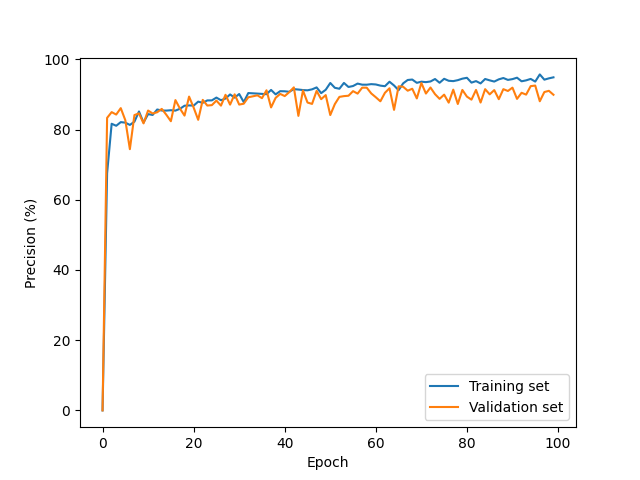
\includegraphics[width=.8\linewidth]{risultati/precision.png}
				\caption{\label{fig:acc2}Training and \\ validation precision}
			\end{minipage}
		\end{figure}
		
		\begin{figure}[!h]
			\centering
			\begin{minipage}{.5\textwidth}
				\centering
				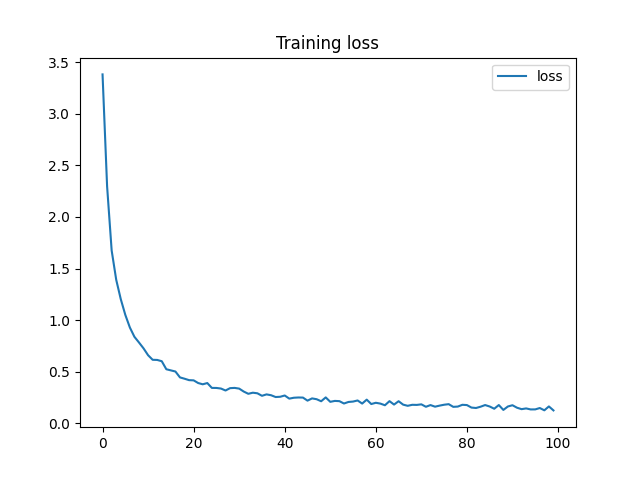
\includegraphics[width=.8\linewidth]{risultati/train_loss.png}
				\caption{\label{fig:loss1}Training loss}
			\end{minipage}%
			\begin{minipage}{.5\textwidth}
				\centering
				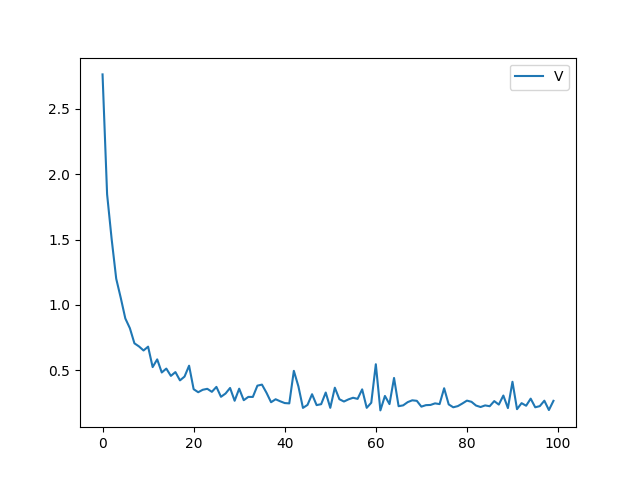
\includegraphics[width=.8\linewidth]{risultati/val_loss.png}
				\caption{\label{fig:loss2}Validation loss}
			\end{minipage}
		\end{figure}
		
		During the experiments phase, we tried some different solutions. 
		Due to the short time we had, though, we could not experiment a lot. 
		The first thing we tried was changing the optimizer's learning rate parameter. 
		The values we used were $0.01$, $0.001$, and $0.0001$. 
		The result was that the best learning rate was, considering the loss value, $0.0001$, even if the difference between that and $0.001$ was very little. 
		Then we tried to understand if the decay had a positive influence on the result. 
		We saw that, without the decay, the model scores slightly better in the test set and slightly worse in the validation set. 
		Then we tried to use different optimizers with the same architecture to see if the results changed. 
		We tried Stochastic Gradient Descent (SGD) with and without Nesterov momentum, RMSprop, Adagrad, and Adadelta. 
		The parameters we used are listed in Table \ref{tab:opt}. 
		The results showed that Adam was the best optimizer. 
		Since the experiment has been shortened due to the lack of time, the optimizers should be studied deeper.
		
		\begin{table}[h]
			
			\caption{\label{tab:opt}Results of the optimizers}
			
			\centering
			\begin{tabular}{|c|c|c|c|c|}
		
				\hline
				\textbf{Optimizer} & \textbf{Parameters} & \textbf{Loss} & \textbf{Accuracy} & \textbf{Precision} \\
				\hline
				SGD & \makecell{learning\_rate = 0.0001 \\ momentum = 0.0 \\ nesterov = False}  & 3.8312 & 0.0525 & 0.0 \\
				\hline
				SGD (Nesterov) & \makecell{learning\_rate = 0.0001 \\ momentum = 0.0 \\ nesterov = True} & 3.9816 & 0.2705 & 0.0\\
				\hline
				RMSProp & \makecell{learning\_rate = 0.0001 \\ rho = 0.9} & 0.2831 & 0.8936 & 0.8939\\
				\hline
				Adadelta & \makecell{learning\_rate = 0.0001 \\ rho = 0.95} & 3.9034 & 0.0289 & 0.0 \\
				\hline
				Adam & \makecell{learning\_rate = 0.0001 \\ decay = 0.0} & 0.1755 & 0.9259 & 0.9263 \\
				\hline
			
			\end{tabular}
	
		\end{table}
		
	\subsection{Consideration about our work}
	
		Due to the short time we had, we could not perform many experiments. 
		The only thing we could experiment on reasonably deep enough was the learning rate for the Adam optimizer. 
		Our work could be considered a starting point. 
		We could prove that player recognition is possible with high accuracy, but many things should still be experimented on or explored.

\section{Results}

	We selected the best model based on the accuracy and precision scored in the validation set. 
	That model achieved very high accuracy and precision, as shown in Table \ref{tab:res}. 
	It has 2 LSTM layers, each of 256 units, two Dropout layers (one after each LSTM layer) with a 0.2 rate, a Dense layer with 128 neurons, and 50 neurons in the output layer. 
	The learning rate was 0.0001. 
	The model's summary is in Figure \ref{fig:best_mod}. 
	This model can generalize very well, and this fact proves that the play style can be biometric in CS:GO.
		
	\begin{table}[!h]
		
		\caption{\label{tab:res}Results of the best model}
	
		\centering
		\begin{tabular}{|c|c|c|c|}
		
			\hline
			 & \textbf{Loss} & \textbf{Accuracy} & \textbf{Precision} \\
			\hline
			Training & 0.1535 & 0.9390 & 0.9392 \\
			\hline
			Validation & 0.1755 & 0.9259 & 0.9263 \\
			\hline
			Test & 0.1975 & 0.9246 & 0.9254 \\
			\hline
			 
		\end{tabular}
		
	\end{table}
	
	\begin{figure}[t!]
		\centering
		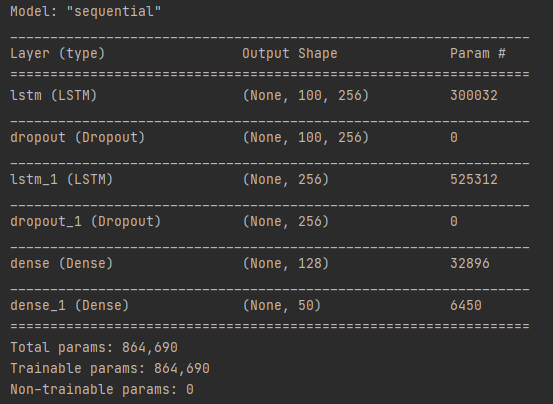
\includegraphics[scale=.6]{modelli/modello_buono.png}
		\caption{\label{fig:best_mod}Summary of the best model.}
	\end{figure}
	
	\null
	\vfill             % Product Prototype
%% !TEX encoding = UTF-8
% !TEX TS-program = pdflatex
% !TEX root = ../tesi.tex

%**************************************************************
\chapter{Discussion}
\label{cap:results}
%**************************************************************

%\intro{In this chapter there is a discussion about our results and how their effects.}\\

%**************************************************************

Being able to recognize a player's play style leads to a lot of different discussions. \\
We firmly believe that this capability is helpful to decrease the number of \gls{Smurf}, \gls{Booster}, and account sellers. 
These three problems are common to the vast majority of online video games. 
In the first case, \gls{Smurf} ruin the experience for the inexperienced players that play with them. 
In the case of \gls{Booster}, there is the opposite problem, since the boosted player is not skilled enough to be on par with the other players he plays with and ruins their match as a consequence. 
Moreover, all the games played by the booster player are ruined, similarly to smurfing. 
Selling an account is problematic because it can result in smurfing or boosting problems.
The capability to punish these people and possibly ban every account they play with is a repellent for the problem. 
The same logic applies to scammers and, more generically, to every form of bad behaviour.
%The DOTA 2 paper, which we took inspiration from, already discussed these possibilities in greater detail. 
Our work proved that there are online video games, a part from DOTA 2, whose players can be identified. 
This opens the door to new studies to see if the play style can be considered biometric also in other video games. 
If even other games offer this possibility, video game publishers can follow this possibility to punish players that commit severe violations of the rules.\\
On the other side, though, a system like this seriously menaces the players' privacy. 
Since some games let a user log in through social media, it is ideally possible to use transfer learning to track gamers among different games and, 
if they logged in through the social media method, take all the public information from the social media used for the authentication.
             % Product Design Freeze e SOP
% !TEX encoding = UTF-8
% !TEX TS-program = pdflatex
% !TEX root = ../tesi.tex

%**************************************************************
\chapter{Final remarks}
\label{cap:conclusioni}
%**************************************************************

\section {Future works}

	In this work, we proved that it is possible to identify a player exploiting the play style in CS:GO. 
	Due to the short time we had, though, we could not experiment a lot. \\
	There are some possible future continuations of this work that aim to extend what we did. 
	One of these is, for example, trying with other neural network architectures and see if changing some hyperparameters (like the number of LSTM units) can benefit the accuracy. 
	Another thing that should be considered is that we worked only with professional players. 
	It would be interesting to see if the accuracy changes if there are non-professional players among the set of selected players. 
	Moreover, we decided to use the same kind of interpolation for all the players but would be interesting to try another type of interpolation or try to adapt the interpolation for every player. 
	Another hint for future experiments could be to study the correlation between the sequence's length and the prediction's accuracy. 
	Once this study is complete, its result could be used to see if other architectures can perform better with shorter sequences. 
	Furthermore, a hint would be trying to understand how to face unknown players. 
	As the last indication, we suggest finding a correlation, if present, between the play style and private data, as in the DOTA 2 work. \\
	As a natural continuation of the work, we suggest trying to involve other video games, possibly belonging to other genres. 
	Finally, some transfer learning techniques can be applied to understand if the play style is game-dependent or not. 

\section{Conclusion}
	
	In this thesis, we proved that deep learning neural networks are able to recognize a player by the play style, which can be considered biometric. 
	The consequences are various, first of all, scammer recognition. 
	Given that this work is the continuation of another study, we indirectly proved that there is more than one video game in which a player's play style can be considered biometric. 
	Being unique for every human, the play style can be used in the authentication process.
             % Discussioni
\input{capitoli/capitolo-8}             % Conclusioni
\appendix                               
% !TEX encoding = UTF-8
% !TEX TS-program = pdflatex
% !TEX root = ../tesi.tex

%**************************************************************
\chapter{Parsing Details\label{app:par}}
%**************************************************************

	In this appendix, we give more details about the parser and how we understood how it works. 
	The original parser we worked on is available on Valve's GitHub page in the repository named csgo-demoinfogo\footnote{\href{https://github.com/ValveSoftware/csgo-demoinfo}{https://github.com/ValveSoftware/csgo-demoinfo}}.
	Since there is no documentation, we had to experiment a lot to understand it. 
	The first thing we noticed is that the parser relies on protobuf messages\footnote{\href{https://github.com/protocolbuffers/protobuf}{https://github.com/protocolbuffers/protobuf}}. 
	After downloading protobuf, we were able to compile the parser and run it. 
	We discovered that the parser logged everything on the console, so we redirected the output to a \emph{txt} file to analyze it. 
	During the analysis of the parser, we noticed that information was saved in some data structures that were called tables by the programmers. 
	The parsing divided entities (which are the players' controlled characters) and actions (performed by the players).
	In Figure \ref{fig:ent}, there is an example of a parsed entity.
	
	\begin{figure}[!h] 
		\centering 
		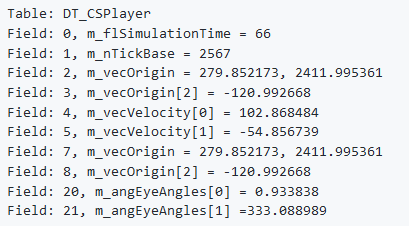
\includegraphics[scale=.8]{parser/original_entity.png}
		\caption{\label{fig:ent}Example of parsed entity.}
	\end{figure}
	
	The first thing we wanted to understand was the logic used, and what the parser saved in the tables. 
	Looking at Figure \ref{fig:ent}, we find some interesting variables dumped. 
	
	\begin{itemize}
	
		\item \texbtbf{Player's position}:\\			
			The variable \texttt{m\_vecOrigin}, contained in 2 couple of fields, contains the player's position relative to the $(0,0,0)$ coordinate of the map. 
			The first field of the couple contains an array of length 2 that memorizes the $X$ and $Y$ coordinate respectively, the other field of the couple memorized the $Z$ coordinate. \\
	
		\item \textbf{Player's speed}:\\
			The variable \texttt{m\_vecVelocity} is an array of length 3 that memorizes the speed of the player along the three axes ($X$, $Y$, and $Z$). 
			It is worth mentioning that at index 0 there is the $X$ axis' speed, at index 1 the $Z$ axis' speed, and at index 2 the $Y$ axis' speed.
	
		\item \textbf{Camera position}:\\
			The variable \texttt{m\_angEyeAngles}, contained in fields 20 and 21, contains two angles (used probably in a 3D polar coordinate system), which represent the position of the mouse and the camera movement. 
			The fact that these variables are angles, thus scaled in a $[0, 360)$ interval, is very useful because results in two variables with equal domain for every user. 
			
	\end{itemize}

	Focusing more on the action, in Figure \ref{fig:act2} there is an example of parsed action.
	
	\begin{figure}[!h] 
		\centering 
		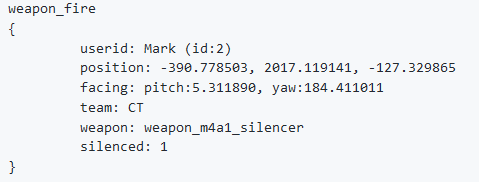
\includegraphics[width=.9\columnwidth]{parser/original_action.png}
		\caption{\label{fig:act2}Example of parsed action.}
	\end{figure}
	
	Focusing on the actions, we thought that every action had a unique id predefined by the game. 
	Parsing different matches, though, we found that the actions' id changed from game to game. 
	At the same time, we noticed that every event has its descriptors, and, in particular, the name used in said descriptors is always the same. 
	We can see, in Figure \ref{fig:act2}, how the action parsed has some properties. 
	The most important is the \texttt{userid}, which represents the id of the user that performed the action. 
	This one, along with the team, are the only common fields through all the actions. 
	Concerning the crouch state, we found that it was treated as an entity property, not as an action. 
	The game keeps track of the offset along the $Y$ axis that represents the crouch state. 
	So we decided to dump the offset and keep track of it as an entity property.\\
	We needed to find a way to keep track of the entity and the actions performed by the player we wanted to analyze. 
	The problem we faced was that entities and actions used two different ids, called \texttt{entityId} and \texttt{id} respectively. 
	So we had to understand how the game gives the id to the player and the entities. 
	We found that it uses the \texttt{steamId}, a unique id in the \gls{Steam} platform. 
	So we decided to create a \emph{.h} file to share the player's data between multiple files. 
	Using this technique, we could share both the \texttt{entityId} and the \texttt{id}, along with all the entity's information, like the position, the speed, the $Y$ offset, and the camera position. 
	This decision helped us to also dump the speed of the player every time the parser output some text since we discovered that the speed was dumped only if there were any changes. 
	Once we created and assigned the values to this file, we modified the parser with some simple if statements. 
	Before every dumping we needed, we checked if the dumped entity was the one we were interested in. 
	In case the parser was dumping an action if the action was one of the ones we wanted  (using the event's name) to keep and if it was performed by the player we were following. 
	With this simple modification, we were able to modify the parser's output and only dump the informations regarding the player we were interested in.
             % Appendice A

%**************************************************************
% Materiale finale
%**************************************************************
\backmatter
\printglossaries
% !TEX encoding = UTF-8
% !TEX TS-program = pdflatex
% !TEX root = ../tesi.tex

%**************************************************************
% Bibliografia
%**************************************************************

\cleardoublepage
\chapter{Bibliography}

\nocite{*}
% Stampa i riferimenti bibliografici
\printbibliography[heading=subbibliography,title={Bibliographic references},type=book]

% Stampa i siti web consultati
\printbibliography[heading=subbibliography,title={Websites},type=online]

% Stampa i paper
\printbibliography[heading=subbibliography,title={Papers},type=inproceedings]

\end{document}
